%\documentclass[11pt,professionalfonts,hyperref={pdftex,pdfpagemode=none,pdfstartview=FitH}]{beamer}
%\usepackage{times}
\documentclass[11pt,professionalfonts]{beamer}
\usefonttheme{serif}
\usepackage{presentation_packages}
\usepackage[version=3]{mhchem}
\DeclareSIUnit\year{yr}
\newcommand{\hilight}[1]{\colorbox{green}{#1}}

\definecolor{mygray}{gray}{0.9}
\definecolor{RoyalBlue}{rgb}{0.25,0.41,0.88}
\def\Emph{\textcolor{RoyalBlue}}

\definecolor{tmp}{rgb}{0.804,0.941,1.0}
\setbeamercolor{numerical}{fg=black,bg=tmp}
\setbeamercolor{exact}{fg=black,bg=red}

\mode<presentation> 
{
  \usetheme{Warsaw}
  \usefonttheme{serif}
  \setbeamercovered{transparent}
}

\setbeamertemplate{footline}%{split theme}
{%
  \leavevmode%
  \hbox{\begin{beamercolorbox}[wd=.5\paperwidth,ht=2.5ex,dp=1.125ex,leftskip=.3cm,rightskip=.3cm plus1fill]{author in head/foot}%
    \usebeamerfont{author in head/foot}\insertshorttitle
  \end{beamercolorbox}%
  \begin{beamercolorbox}[wd=.5\paperwidth,ht=2.5ex,dp=1.125ex,leftskip=.3cm,rightskip=.3cm]{title in head/foot}
%    \usebeamerfont{title in head/foot}\mypaper\hfill \insertframenumber/\inserttotalframenumber
    \usebeamerfont{title in head/foot}\hfill \insertframenumber/\inserttotalframenumber
  \end{beamercolorbox}}%
  \vskip0pt%
} \setbeamercolor{box}{fg=black,bg=yellow}


\title[Asteroid Reconstruction]{\large\textbf Real Time Adaptive Shape Reconstruction for Asteroid Landing}

\author{\vspace*{-0.3cm}}
   
\institute{
	\footnotesize
	{\normalsize\bf{Shankar Kulumani}}\\
	\vspace*{0.2cm}
  	\textbf{Department of Mechanical \& Aerospace Engineering}\\ \vspace*{0.5cm}
 	\begin{figure} %figure%
       	
\includegraphics[width=0.75\textwidth]{gw_txh_2cs_pos}
  	\end{figure}
}
\date{20180421}

\begin{document}
%=======================================================%

\setcounter{framenumber}{-1}
\begin{frame} %-----------------------------%
  \titlepage
\end{frame}   %-----------------------------%

\section*{}
\subsection*{Introduction}  
\begin{frame}{Asteroid Missions}
\begin{itemize}
    \item<1-> Science - insight into the early formation of the solar system
    \item<2-> Mining - vast quantities of useful materials
    \item<3-> Impact - high risk from hazardous near-Earth asteroids
\end{itemize}    

\visible<1->{
\begin{center}
    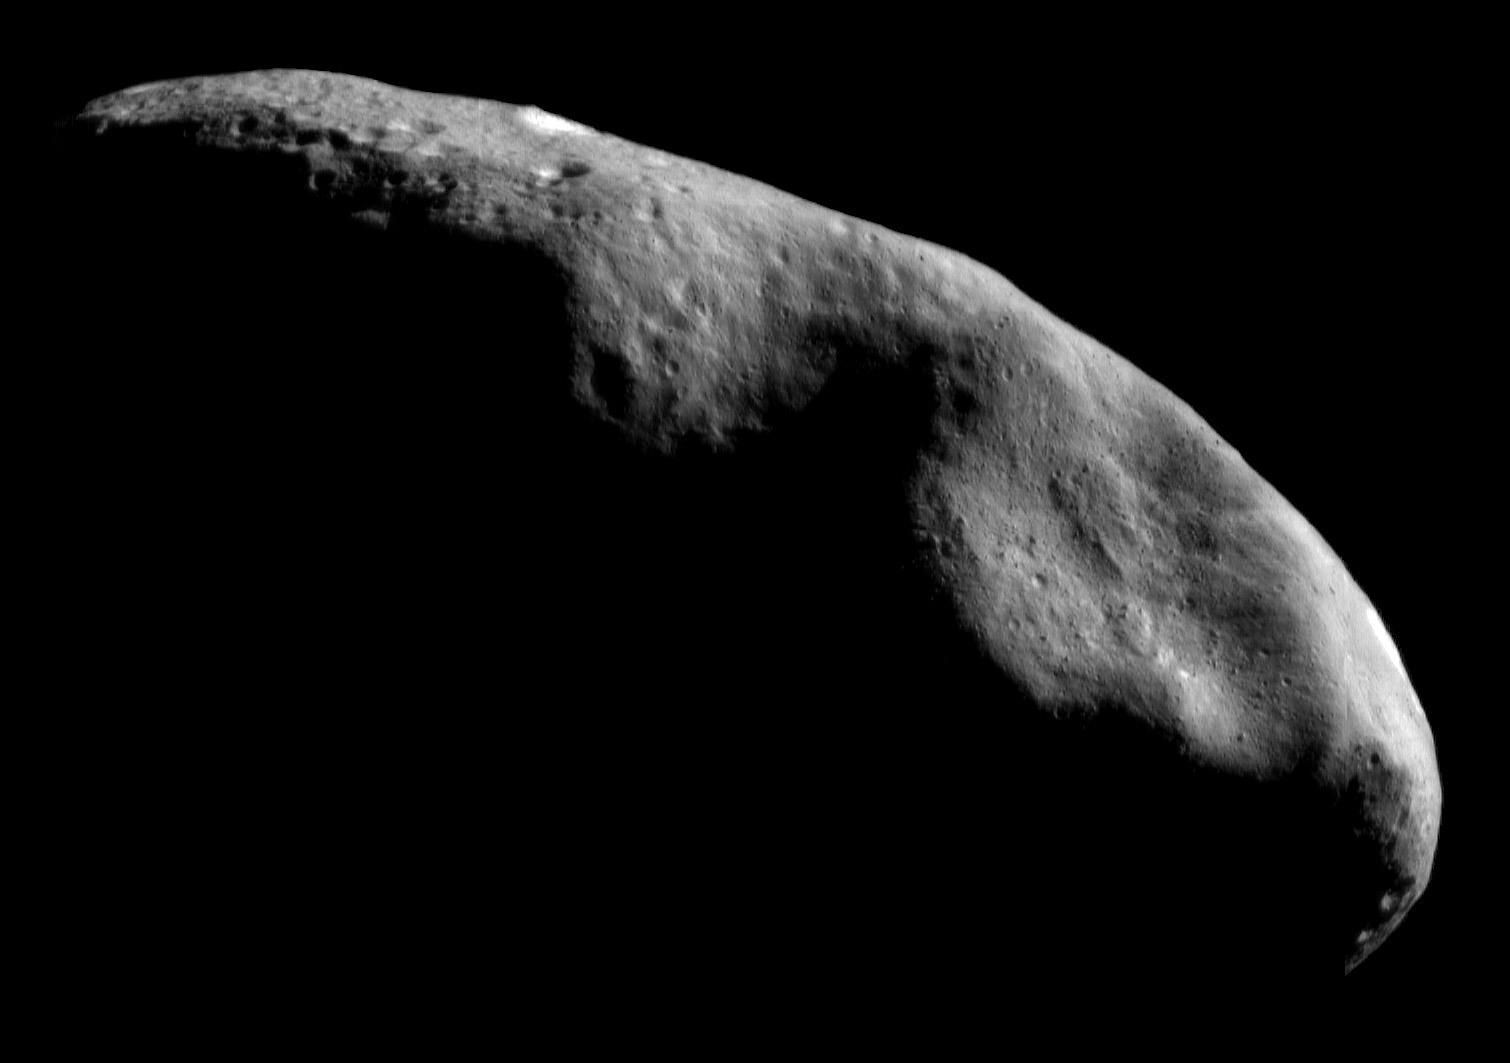
\includegraphics[height=0.35\textheight]{figures/near_mos_20001203_full.jpg}
    \hfill
    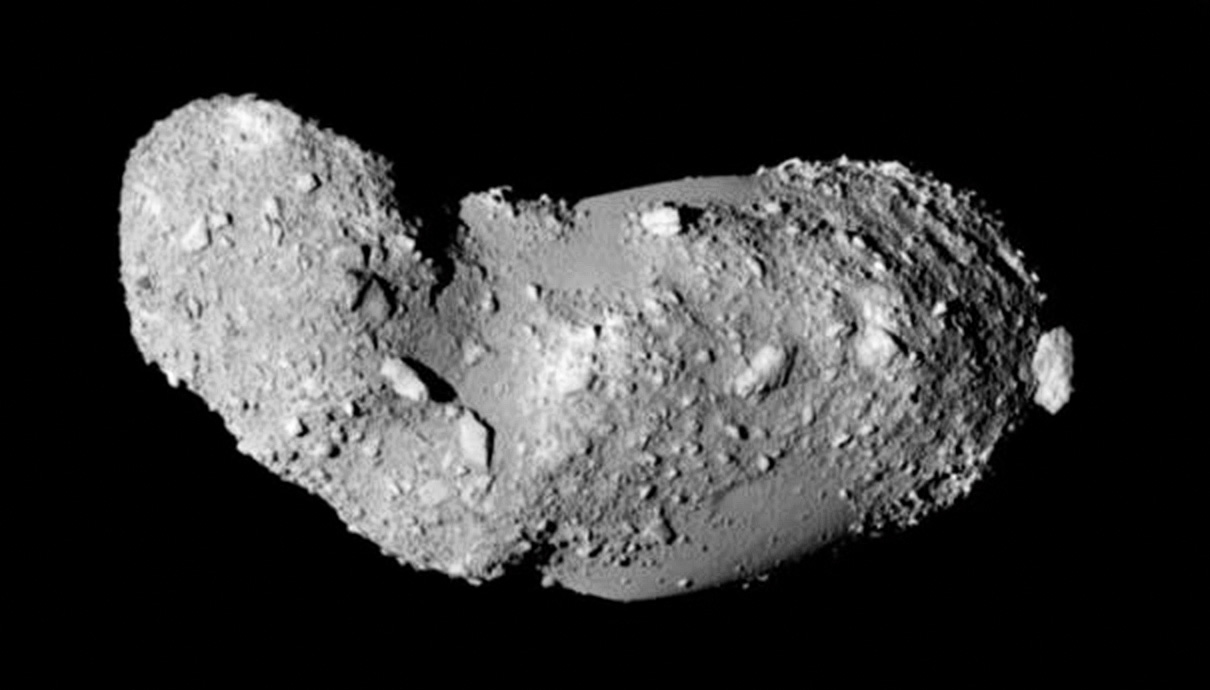
\includegraphics[height=0.35\textheight]{figures/Itokawa8_hayabusa_1210.jpg}
\end{center}
}
\end{frame}

\begin{frame}{Asteroid Mining}
    \begin{itemize}
      \item Useful materials can be extracted from asteroids to support:
      \begin{itemize}
          \item Propulsion, construction, life support, agriculture, and precious/strategic metals
      \end{itemize}
        \pause
      \item Commercialization of near-Earth asteroids is feasible
    \end{itemize}


\begin{center}
\small
    \begin{tabular}{|l|r|r|}
        \hline 
        Element & Price (\SI{}[\$\,]{\per\kilo\gram}) & Sales (\SI{}[\$\,]{M\per\year}) \\
        \hline \hline 
        Phosphorous (P) & \num{0.08}  & \num{2167} \\
        Gallium (Ga) & \num{300.00}  & \num{1544} \\
        Germanium (Ge) & \num{745.00} & \num{6145} \\
        \hline \hline 
        Platinum (Pt) & \num{12394.00} & \num{1705} \\
        Gold (Au) & \num{12346.00} & \num{49} \\
        Osmium (Os) & \num{12860.00} & \num{307} \\
        \hline
    \end{tabular}
\end{center}

\end{frame}

\section*{}
\subsection*{Motivation}  
\begin{frame}{Asteroid Landing}
    \begin{itemize}
        \item Long history of asteroid/planetary missions
            \begin{itemize}
                \item NEAR, Hayabusa, OSIRIS-REX, Rosetta
            \end{itemize}
            \pause
        \item Asteroid landing is particularly challenging:
            \begin{itemize}
                \item<2-> Challenging dynamics - unknown gravity enviornment
                \item<2-> Poor shape model - unknown surface topography
                \item<2-> Attitude coupling - pertubations are large 
            \end{itemize}
    \end{itemize}
    \begin{center}
        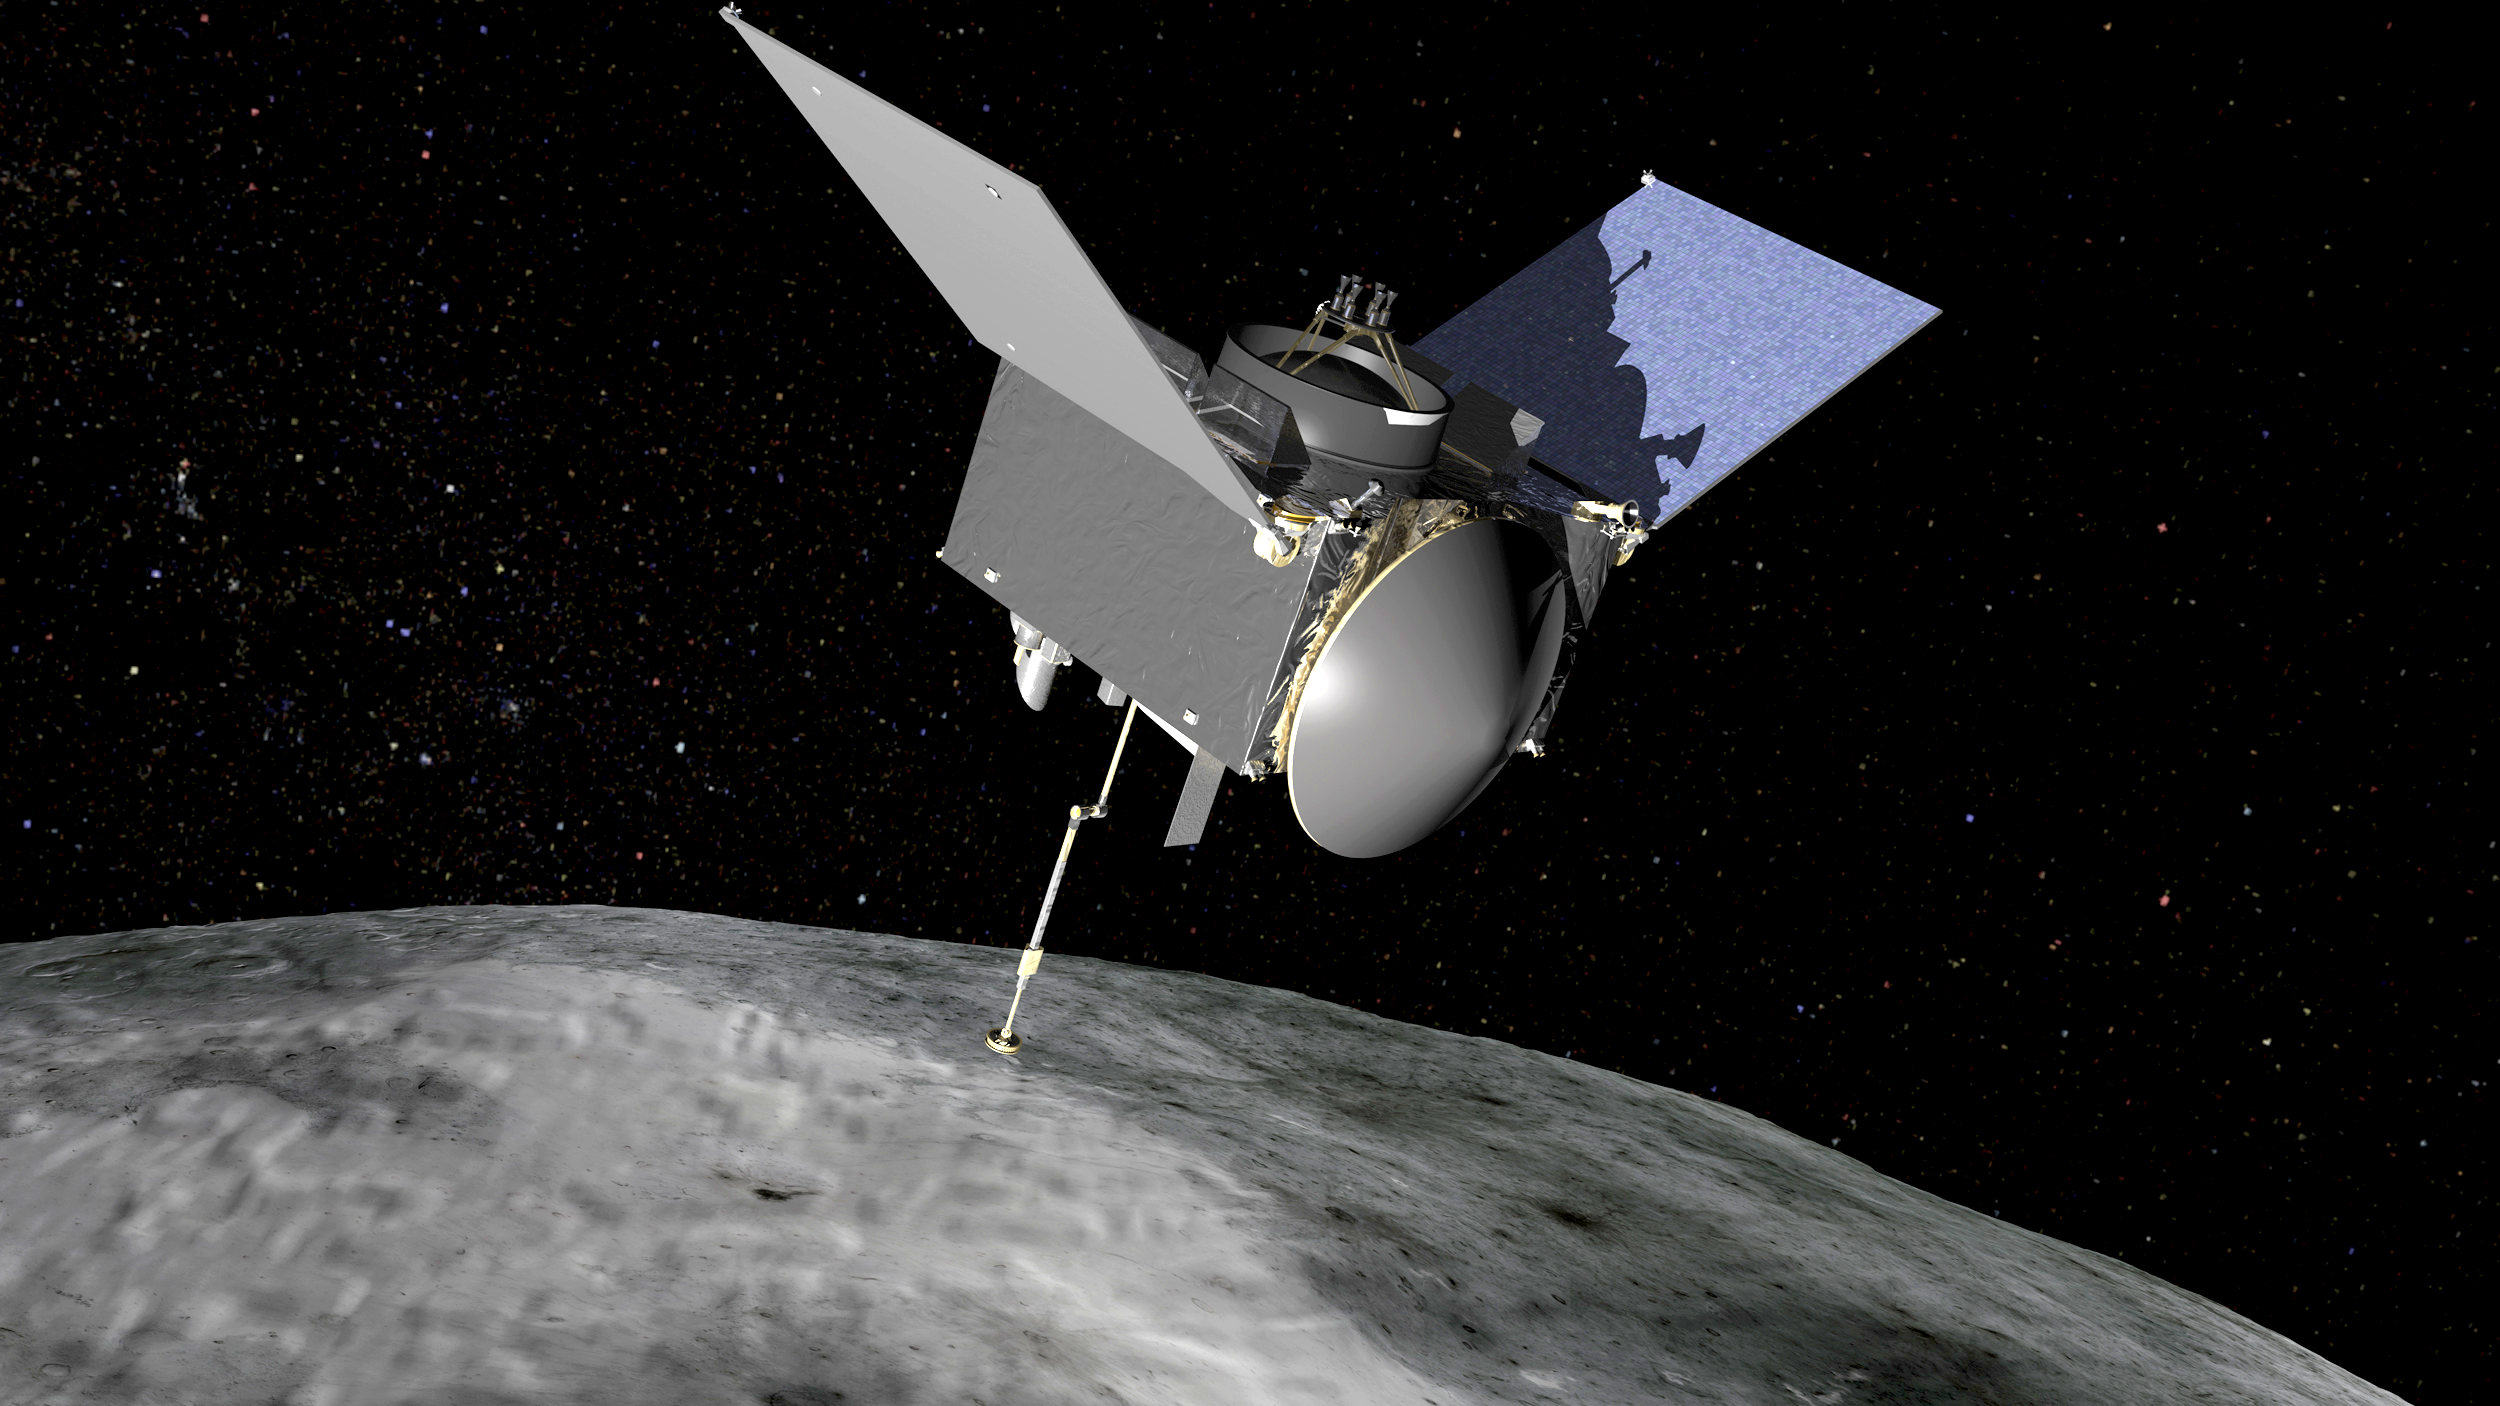
\includegraphics[width=0.6\textwidth,height=0.4\textheight,keepaspectratio]{figures/osiris_rex.png}~
        \includegraphics[width=0.6\textwidth,height=0.4\textheight,keepaspectratio]{figures/Rosetta_Philae_Artist_Impression_Close_4k.jpg}
    \end{center} 
\end{frame}

\begin{frame}{Challenges in Asteroid Missions}
    \begin{itemize}
        \item<1->  Challenging dynamic enviornment
            \begin{itemize}
                \item<1-> Highly irregular shape and chaotic spin states
                \item<1-> Difficult to identitfy and track from the ground
                \item<1-> Poor understanding upon spacecraft arrival
            \end{itemize}
        \item<2-> Coupled translational and rotational dynamics
            \begin{itemize}
                \item Spacecraft is relatively large compared to the orbit radius
                \item Complex interaction between the attitude and position forces
                \item Magnified at lower altitudes and with highly irregular shapes
            \end{itemize}
        \item<3-> Gravity is the primary perturbing force
            \begin{itemize}
                \item Polyhedron potential model is the standard approach 
                \item Accurate shape model is critical for accurate gravity model
                \item In situ measurements are required for accurate shape model
            \end{itemize}
    \end{itemize}
   
    \onslide<3>{
        \begin{block}{}
            \begin{center}
            Shape Model \( \to \) Gravity Model
        \end{center}
        \end{block}
    }
\end{frame}

\begin{frame}{Asteroid Shape Modeling}
    \begin{itemize}
        \item<1-> Ground radar used to compute the 3D shape of the asteroid
        \begin{itemize}
            \item Computationally intensive estimation algorithm 
            \item The result is still coarse and only an approximation
            \item Not accurate enough for low altitude or landing operations
        \end{itemize}
    \item<2-> Estimating the asteroid shape is the first step of any mission
    \begin{itemize}
        \item Months or years are devoted solely to measuring the surface
        \item Laser ranging used to accurately measure relative distance
        \item All data is sent to the ground for processing
    \end{itemize}
    \end{itemize}
    
    \onslide<3->{
        \begin{block}{}
            \begin{center}
                Real-time on board shape estimation
            \end{center}
        \end{block}
    }
\end{frame}

\begin{frame}{Problem Statement}
\begin{enumerate}
    \item<1-> Compute the surface shape from range measurements
        \begin{itemize}
            \item Real time and incrementally build the shape
        \end{itemize}
    \item<2-> Utilize shape model in dynamics and controller
        \begin{itemize}
            \item Coupled equations of motion 
            \item Nonlinear controller for maneuvering and landing
        \end{itemize}
    \item<3-> Autonomously navigate around asteroid 
        \begin{itemize}
            \item Locate areas of poor knowledge for additional measurements
            \item Avoid obstacles or hazards
        \end{itemize}
\end{enumerate}
\end{frame}

\section*{}
\subsection*{Mathematical Background}
\begin{frame}{Polyhedron Gravitation Model}

\begin{itemize}
    \item Potential is a function of only the shape model
    \item Globally valid, closed-form expression of potential
    \item Exact potential assumes a constant density 
    \item Accuracy solely dependent on shape model
\end{itemize}

\visible<2>{
\begin{align*}
    U(\vecbf{r}) &= \frac{1}{2} G \sigma \sum_{e \in \text{edges}} \vecbf{r}_e \cdot \vecbf{E}_e \cdot \vecbf{r}_e \cdot L_e - \frac{1}{2}G \sigma \sum_{f \in \text{faces}} \vecbf{r}_f \cdot \vecbf{F}_f \cdot \vecbf{r}_f \cdot \omega_f 
\end{align*}
}
\begin{center}
    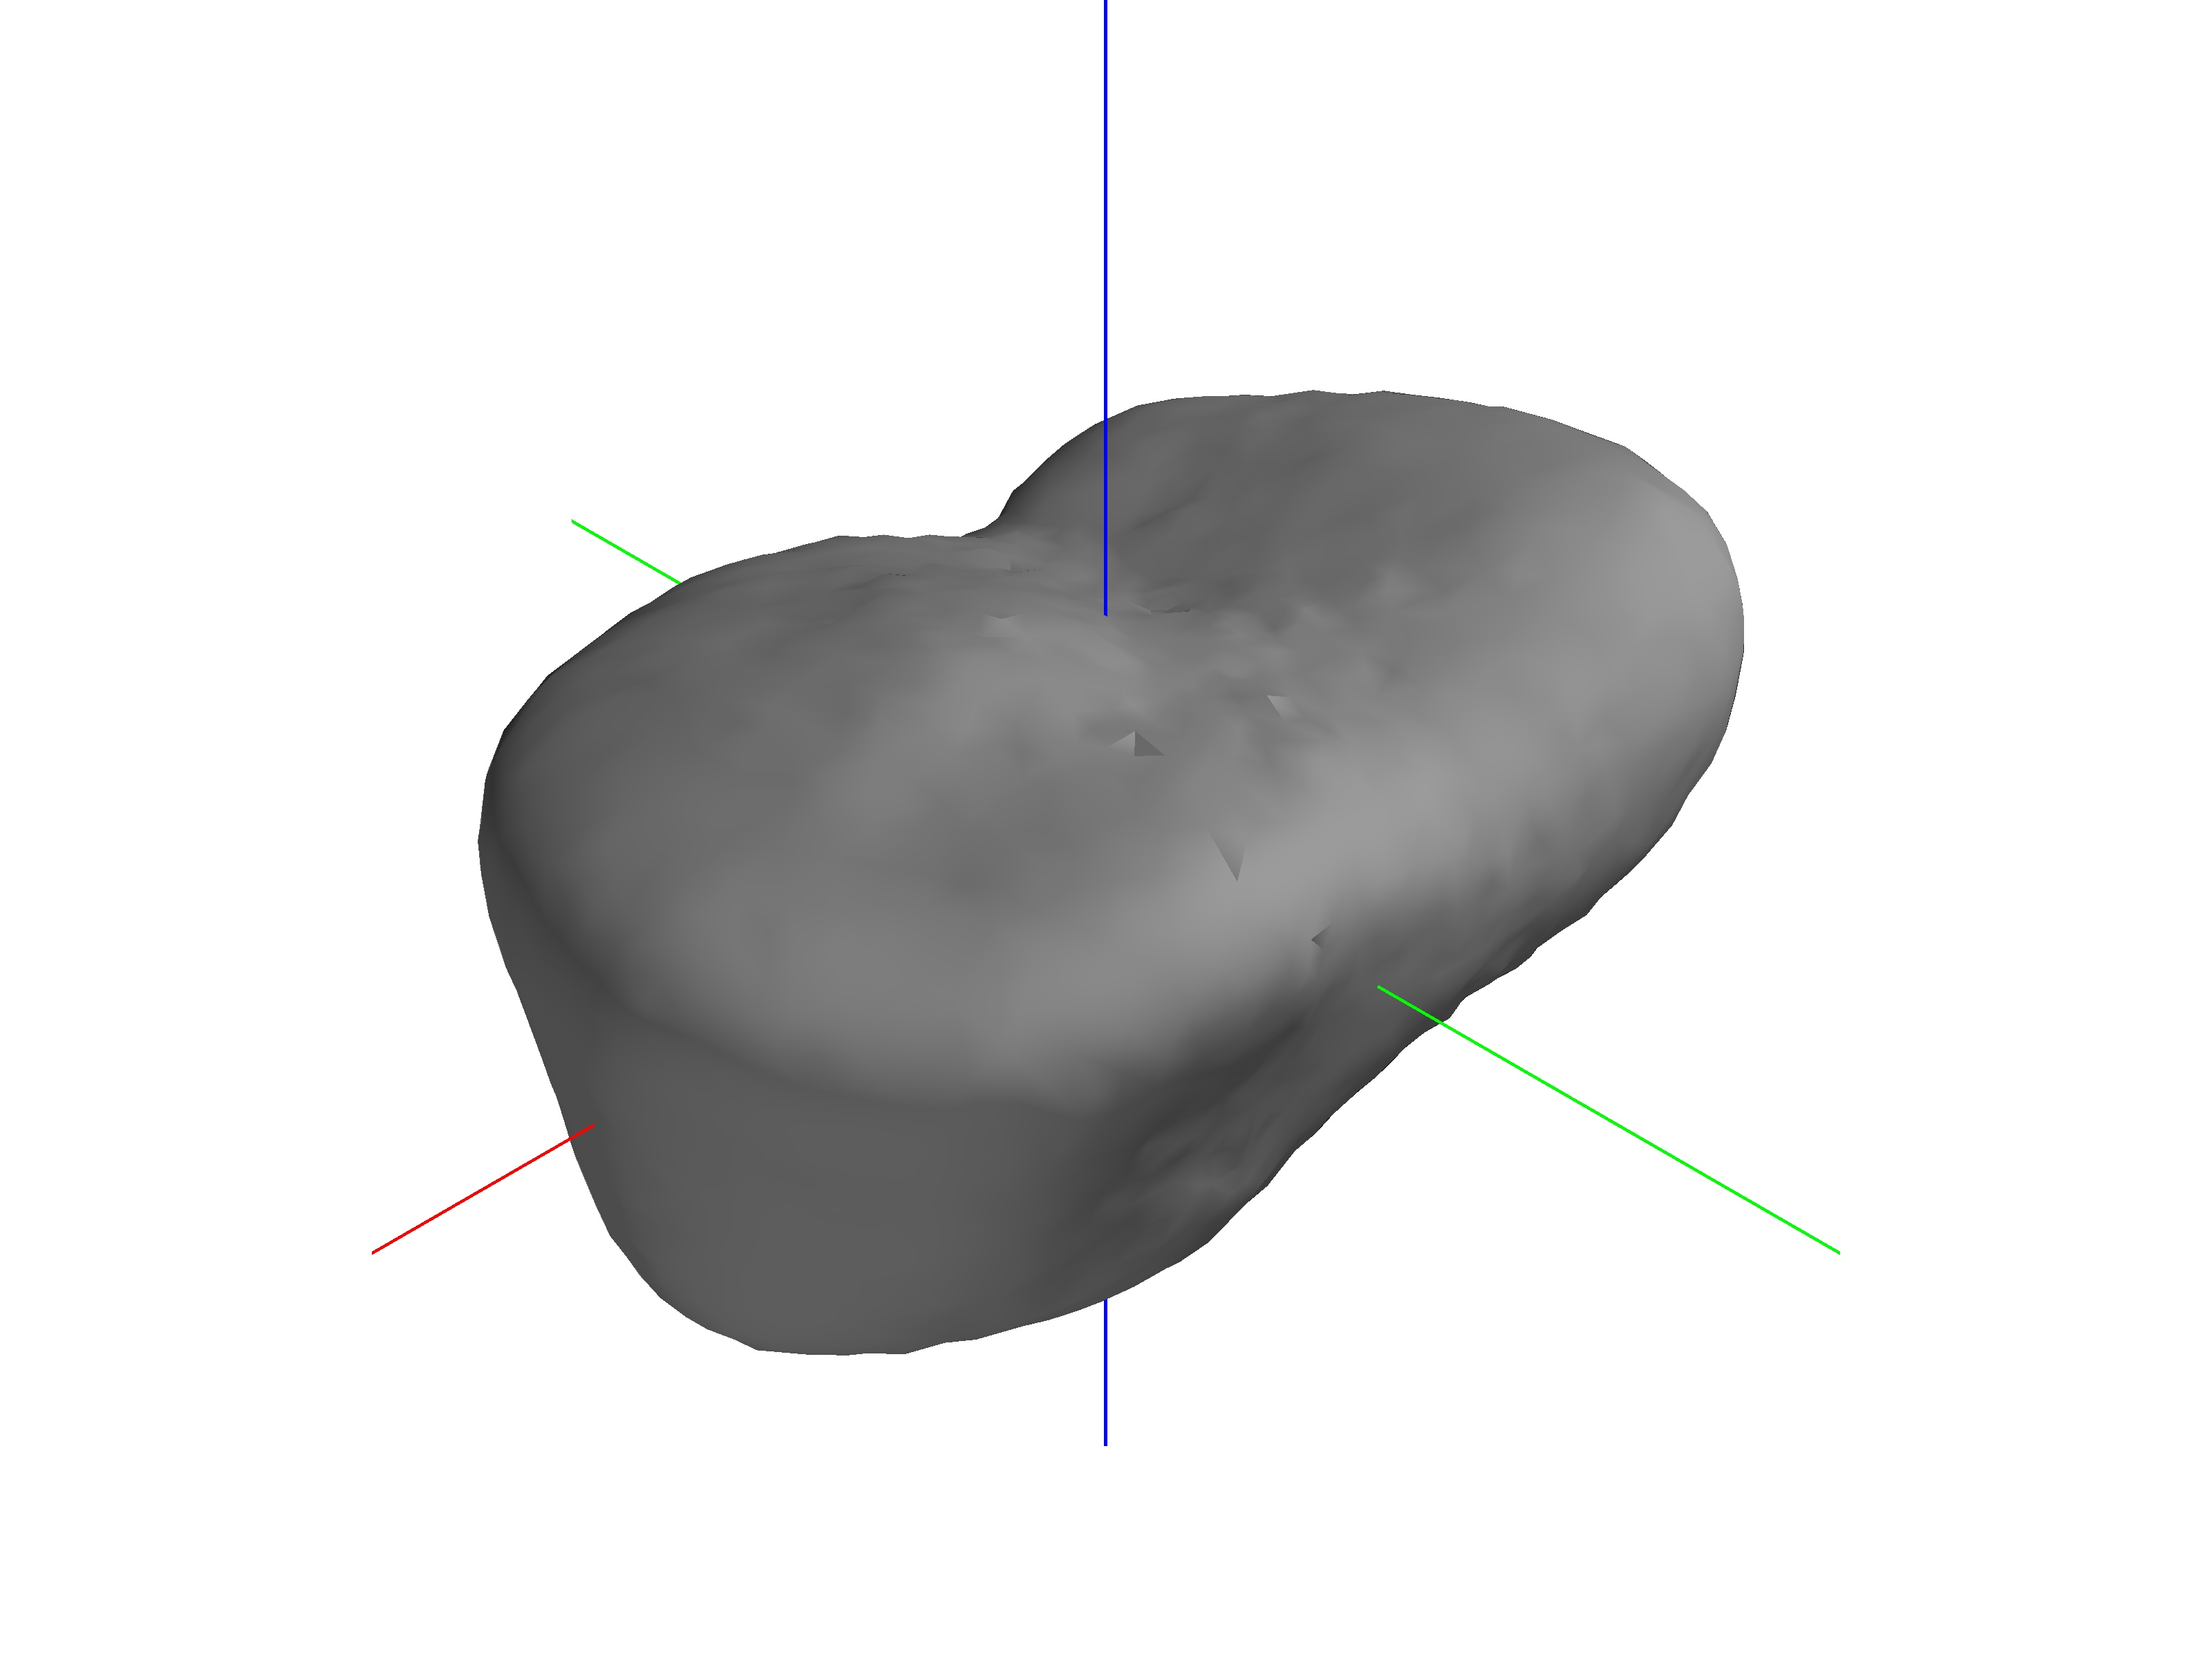
\includegraphics[width=0.5\textwidth,keepaspectratio]{figures/castalia/partial_2047.jpg}~
    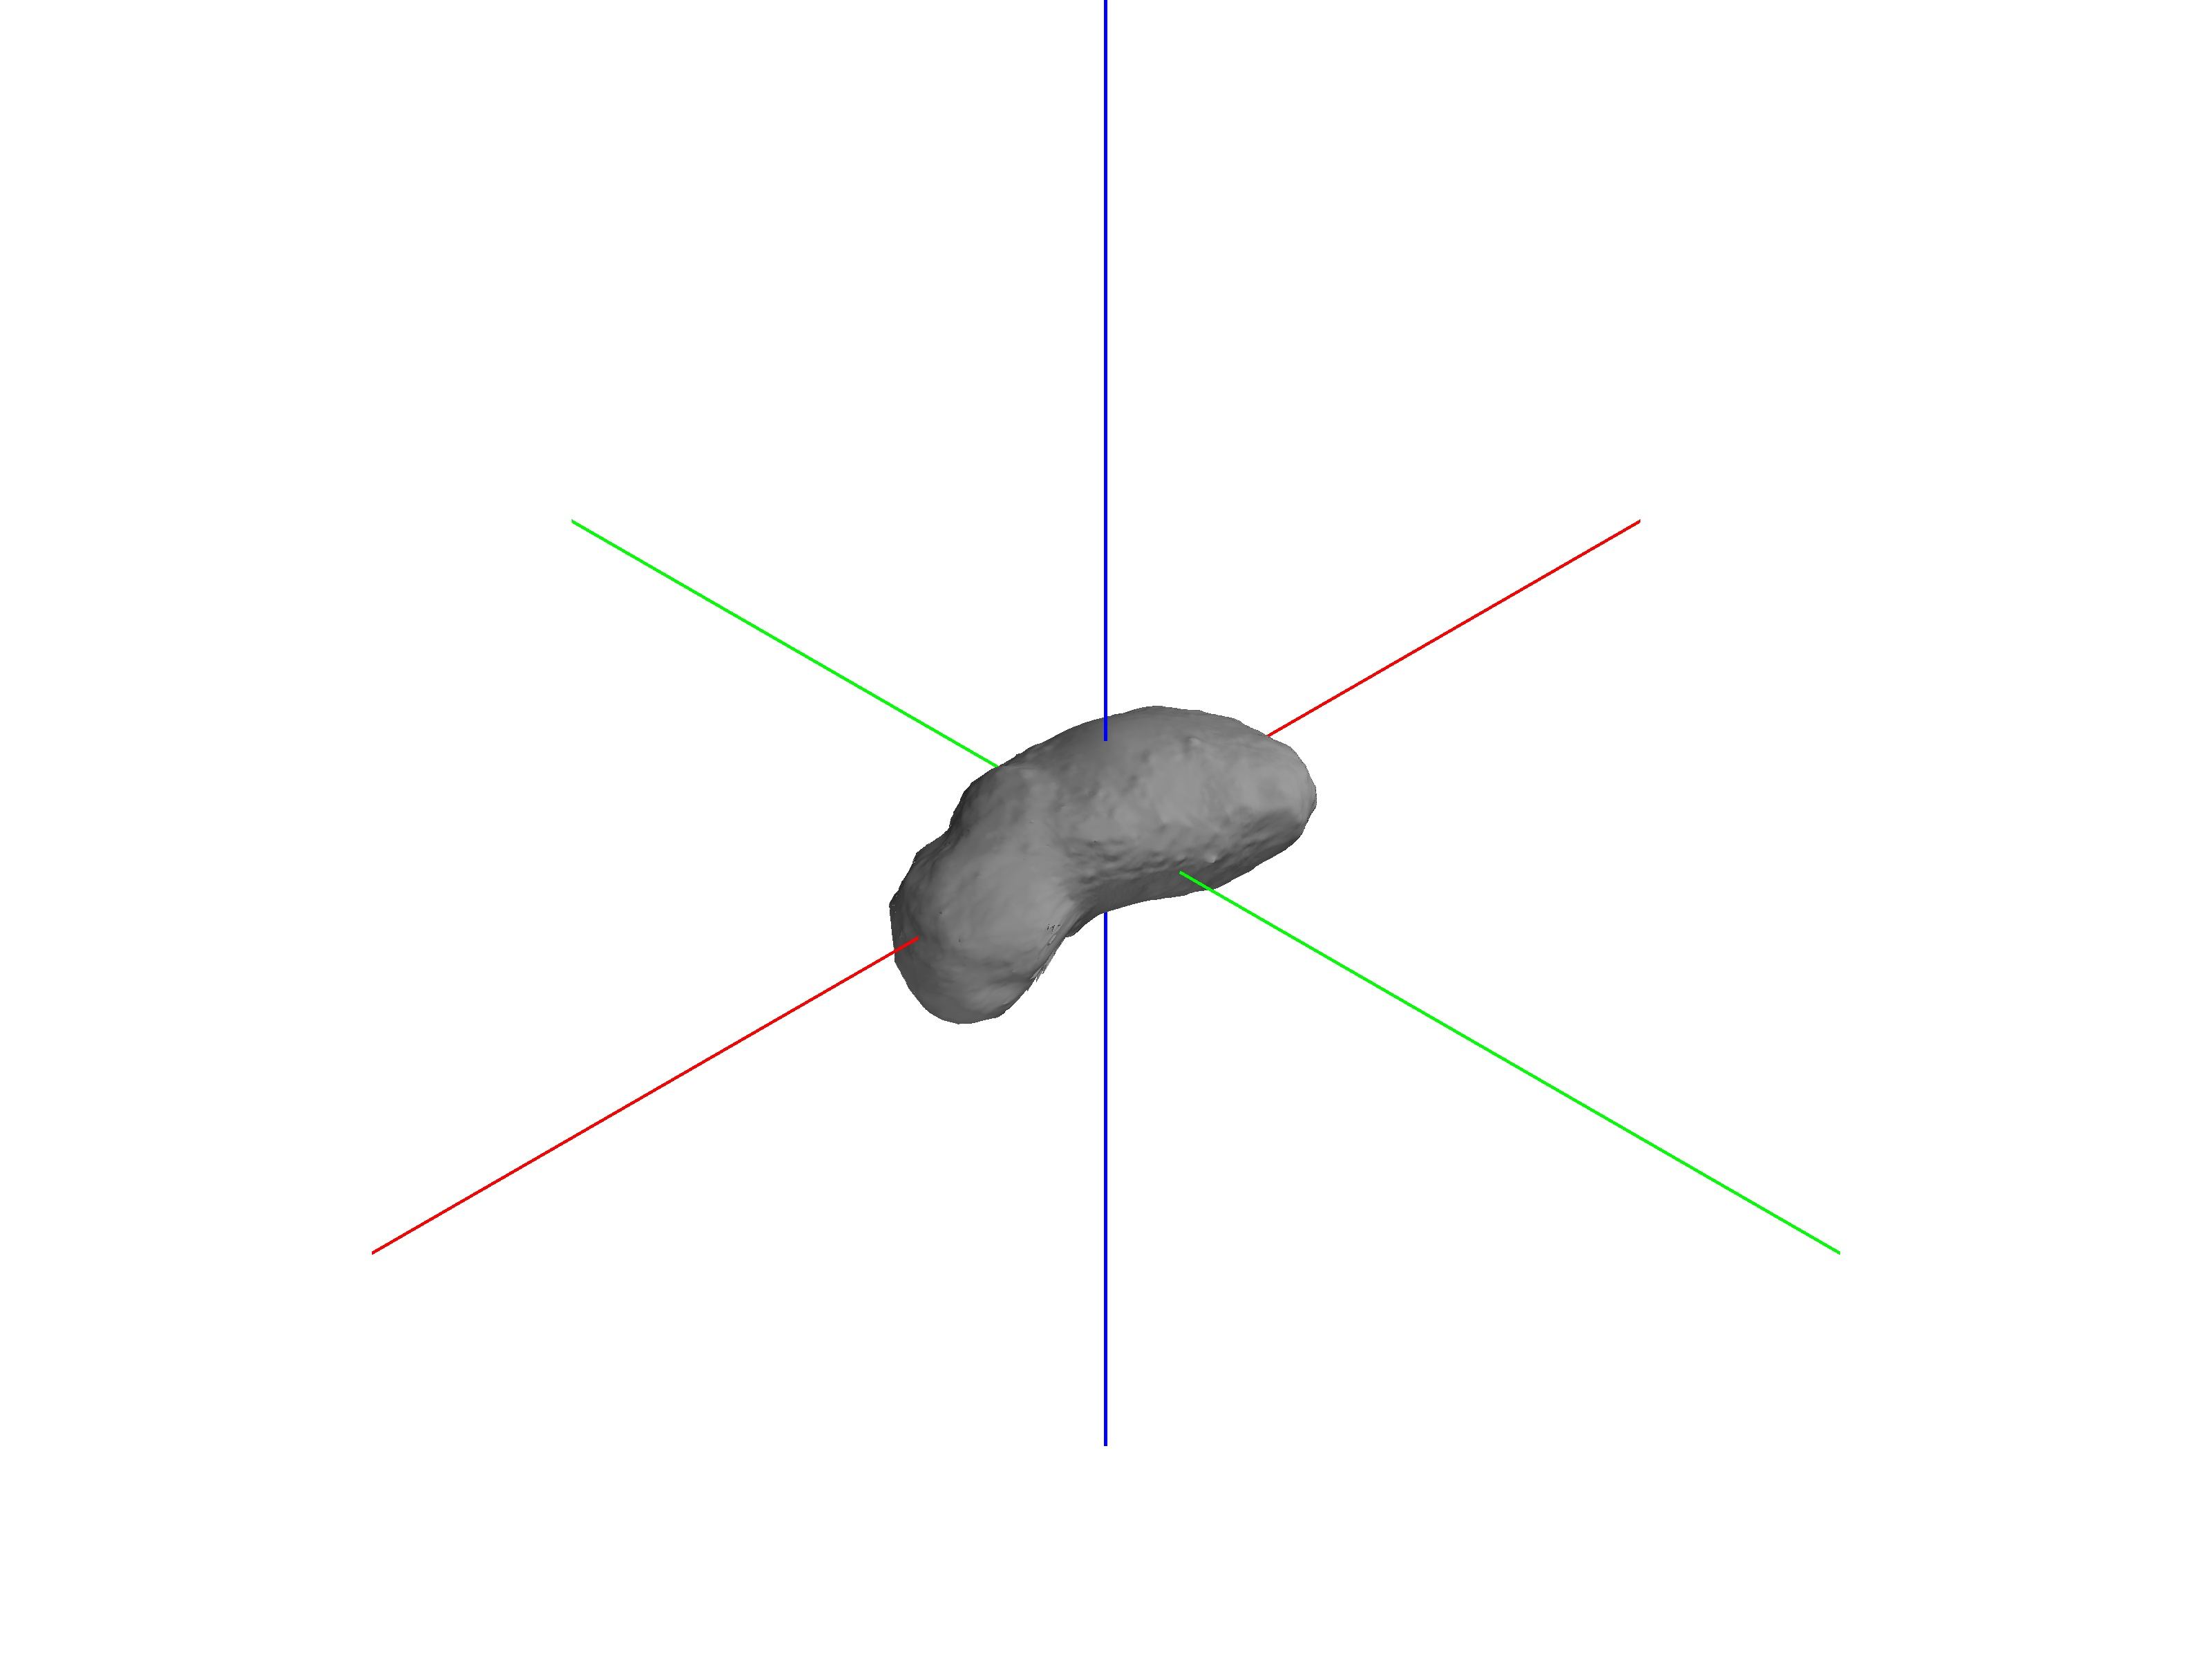
\includegraphics[width=0.5\textwidth,keepaspectratio]{figures/itokawa/partial_25349.jpg}
\end{center}
\end{frame}

\begin{frame}{LIDAR Measurements }
    \begin{itemize}
        \item<1-> Laser pulse used to measure relative distance to surface
        \item<2-> Accurate timing gives the round trip time of flight
            \begin{align*}
                d = \frac{\Delta t}{2 c}
            \end{align*}
    \end{itemize}
    
    \visible<2->{
    \begin{center}
        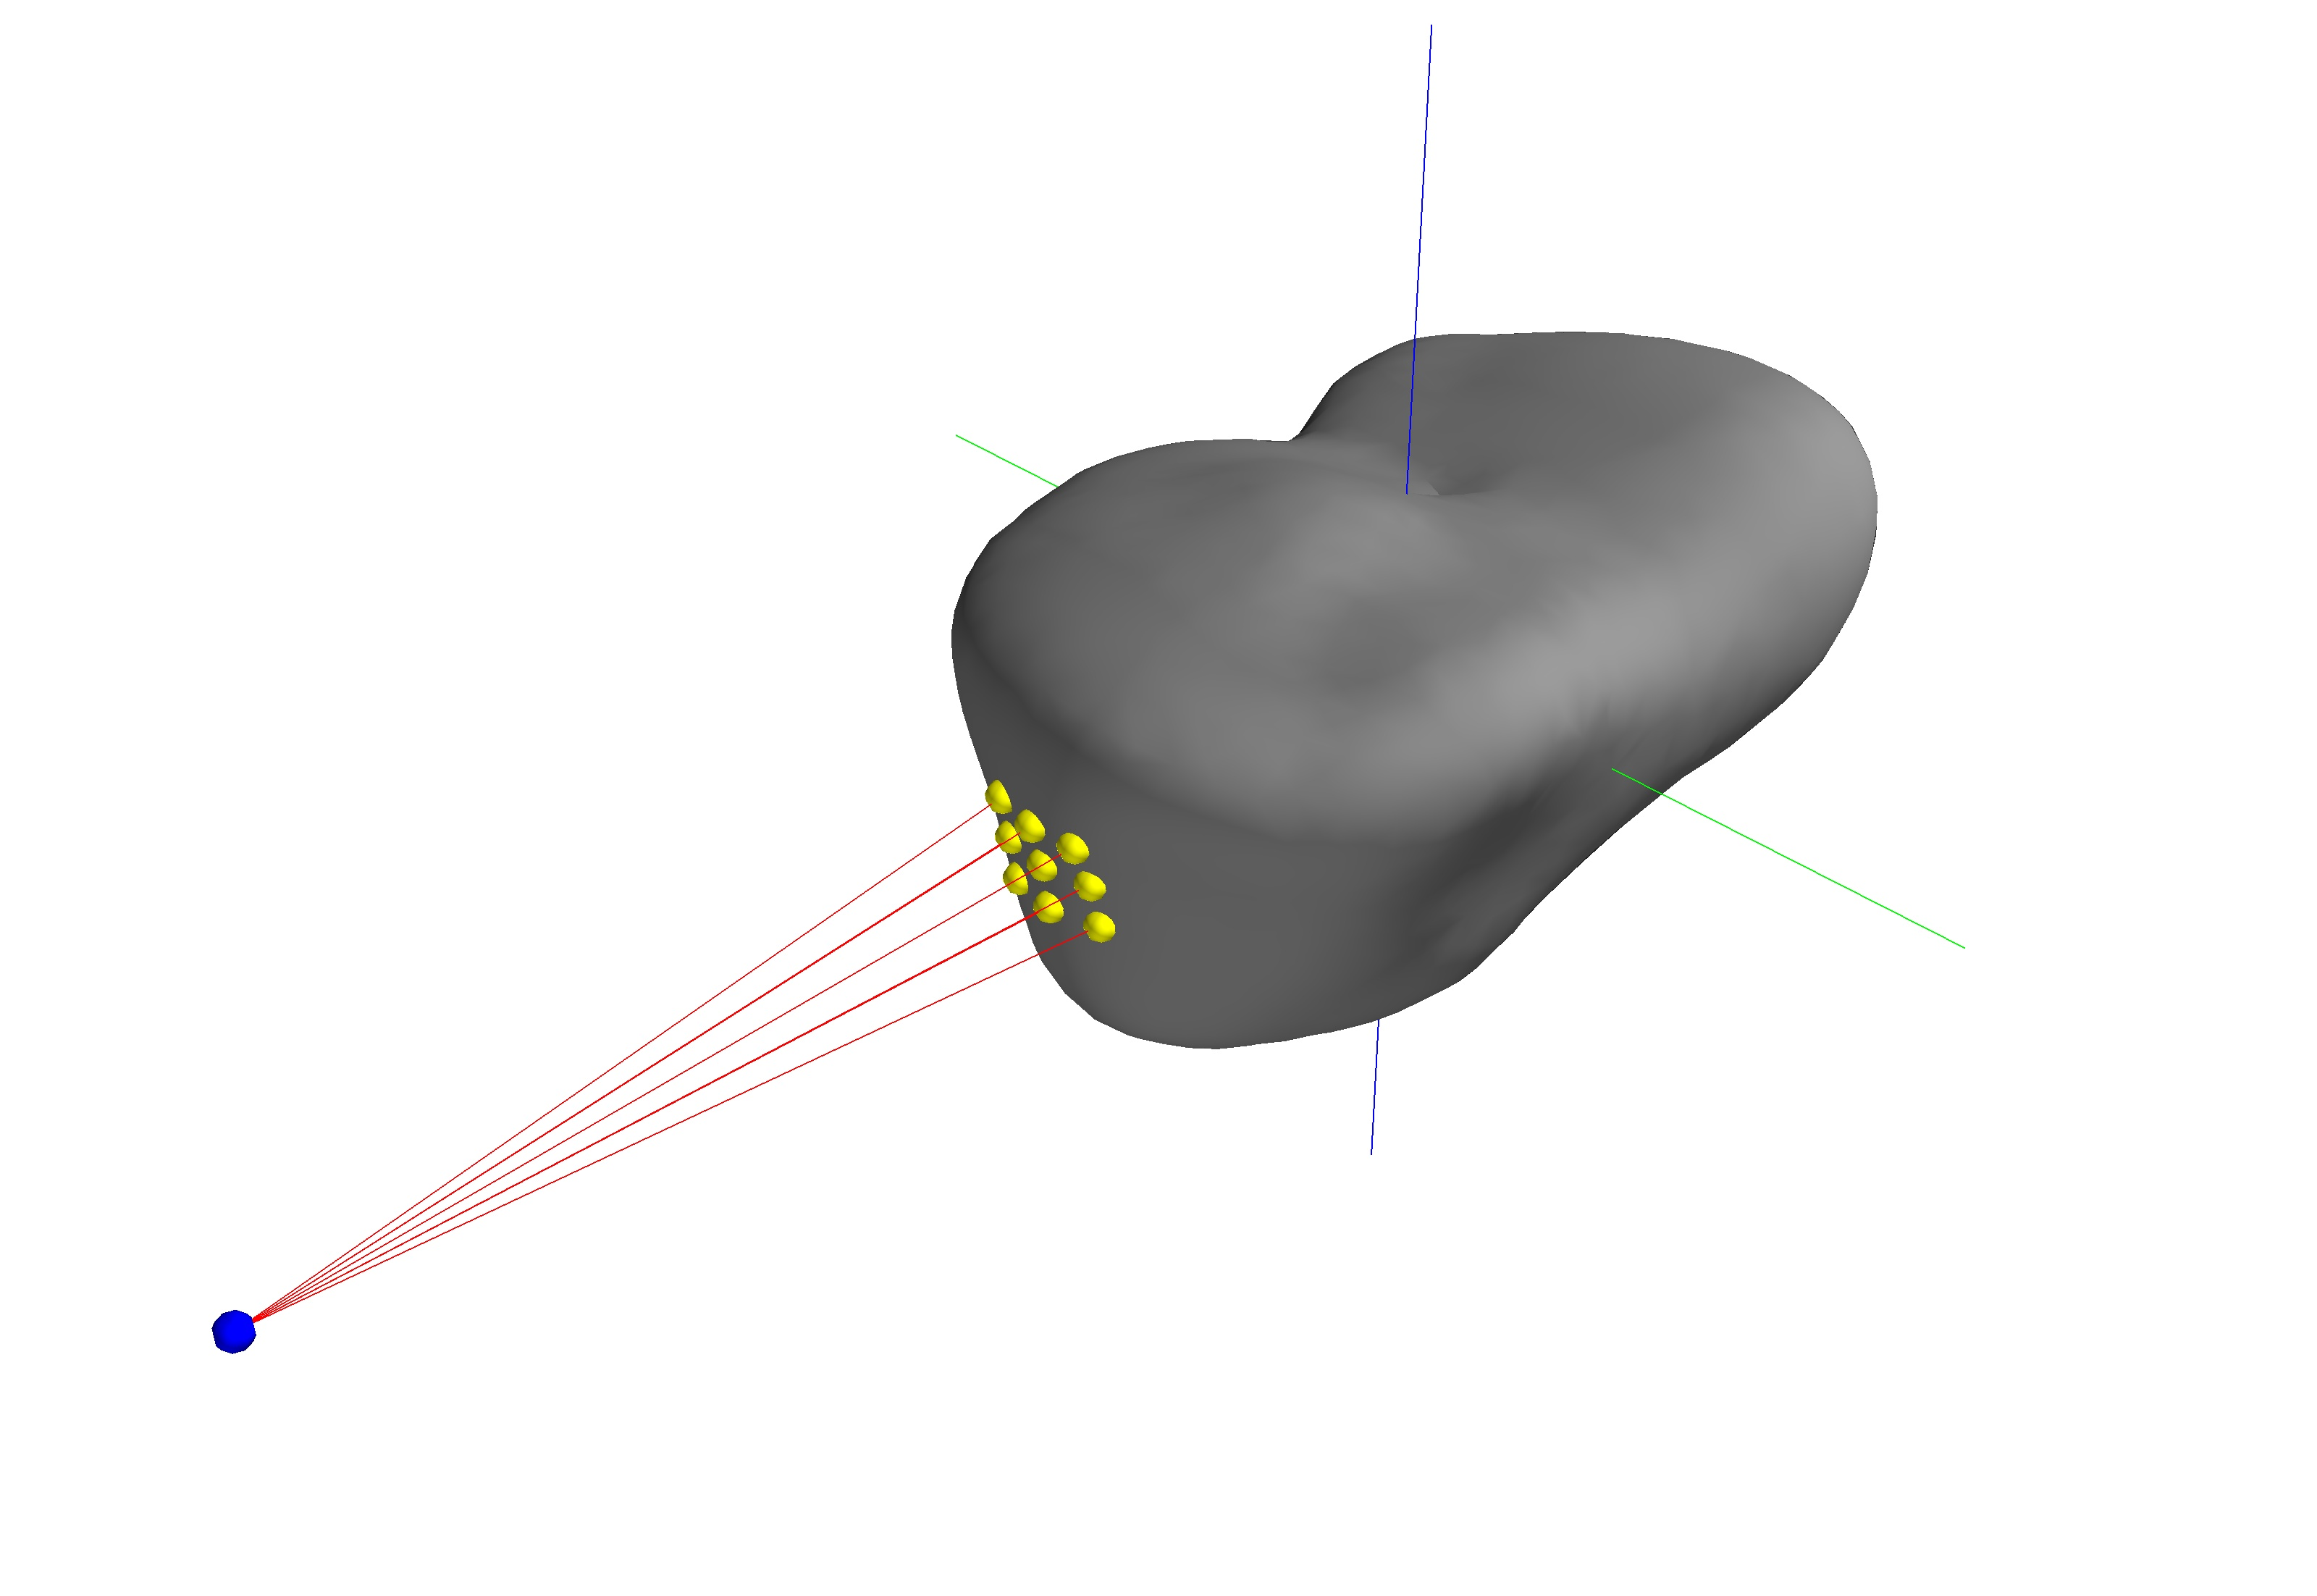
\includegraphics[width=0.75\textwidth]{figures/castalia_raycasting_plot.jpg}
    \end{center}
}
\end{frame}

\begin{frame}{Bayesian Shape Reconstruction}
    \begin{itemize}
        \item<1-> Framework for combining prior and new data 
            \begin{itemize}
                \item Each vertex has an uncertainty -- \( w_i\)
                \item Each measurement has contains some error -- \( w_{j, i} \)
            \end{itemize}
            \begin{align*}
                v_i \sim \mathcal{N}(r_i, w_i^2) , \quad
                p_{j,i} \sim \mathcal{N}(r_{j,i}, w_{j,i}^2)
            \end{align*}
        \item<2-> New data used to update each vertex and reduce uncertainty
    \begin{align*}\label{eq:posterior_probability}
        \mathcal{N} \parenth{\frac{w_{j, i}^2 r_i + w_i^2 r_{j, i}}{w_i^2 + w_{j, i}^2} , \frac{w_i^2  w_{j, i}^2}{w_i^2 +  w_{j, i}^2}} .
    \end{align*}
    \end{itemize}
\end{frame}

\section*{}
\subsection*{Numerical Results}

\begin{frame}{4769 Castalia reconstruction}
    \begin{center}
        \movie[width=0.8\textwidth,height=0.8\textheight,externalviewer]{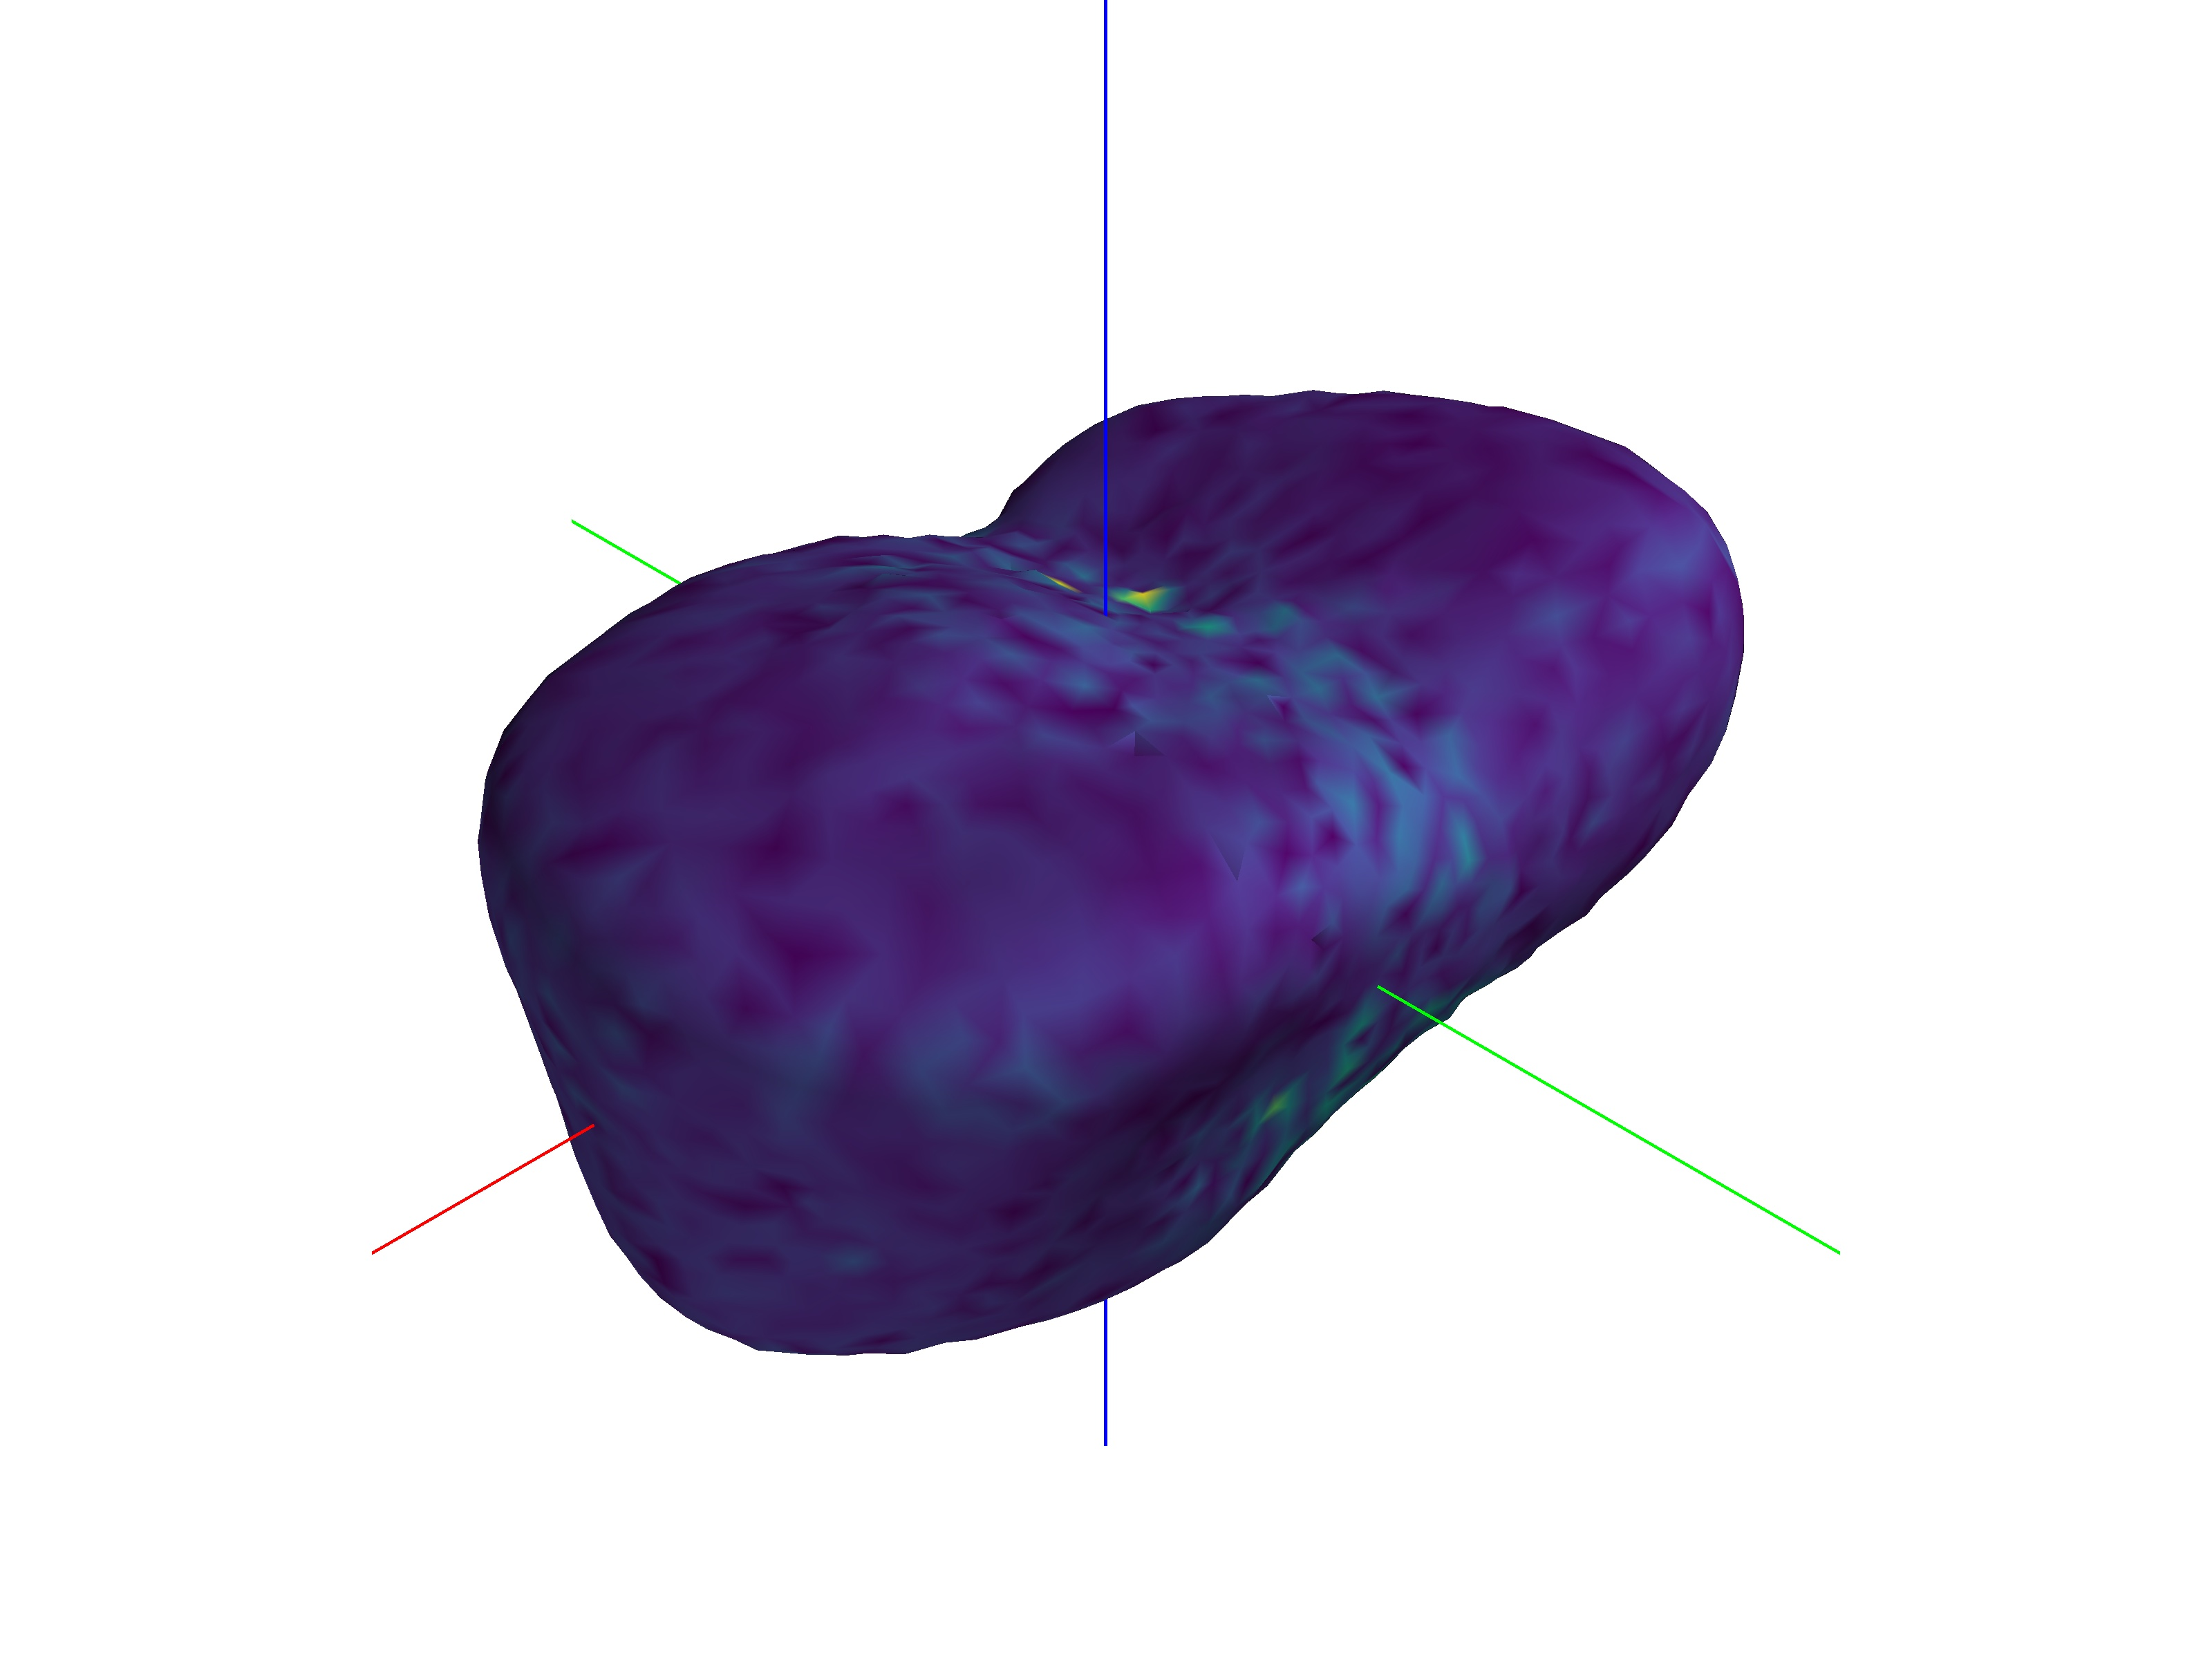
\includegraphics[width=0.8\textwidth,height=0.8\textheight, keepaspectratio]{figures/castalia/partial_weights_2047.jpg}}{./videos/castalia.mp4}
\end{center}
\end{frame}

\begin{frame}{4769 Castalia}
    \begin{columns}
        \begin{column}{0.5\textwidth}
            \centering
            \includemedia[
            label=castalia,
            3Dviews=animation/castalia.vws,
            width=0.5\textwidth,height=0.6\textheight,
            3Dmenu, 
            3Dc2c=-1 0 0,
            3Dcoo=0.04557958245277405 -0.03455224633216858 -0.017790749669075012,
            3Droo=4.029169586482155,
            3Dlights=Headlamp,
            % add3Djscript=animation/castalia.js
            ]{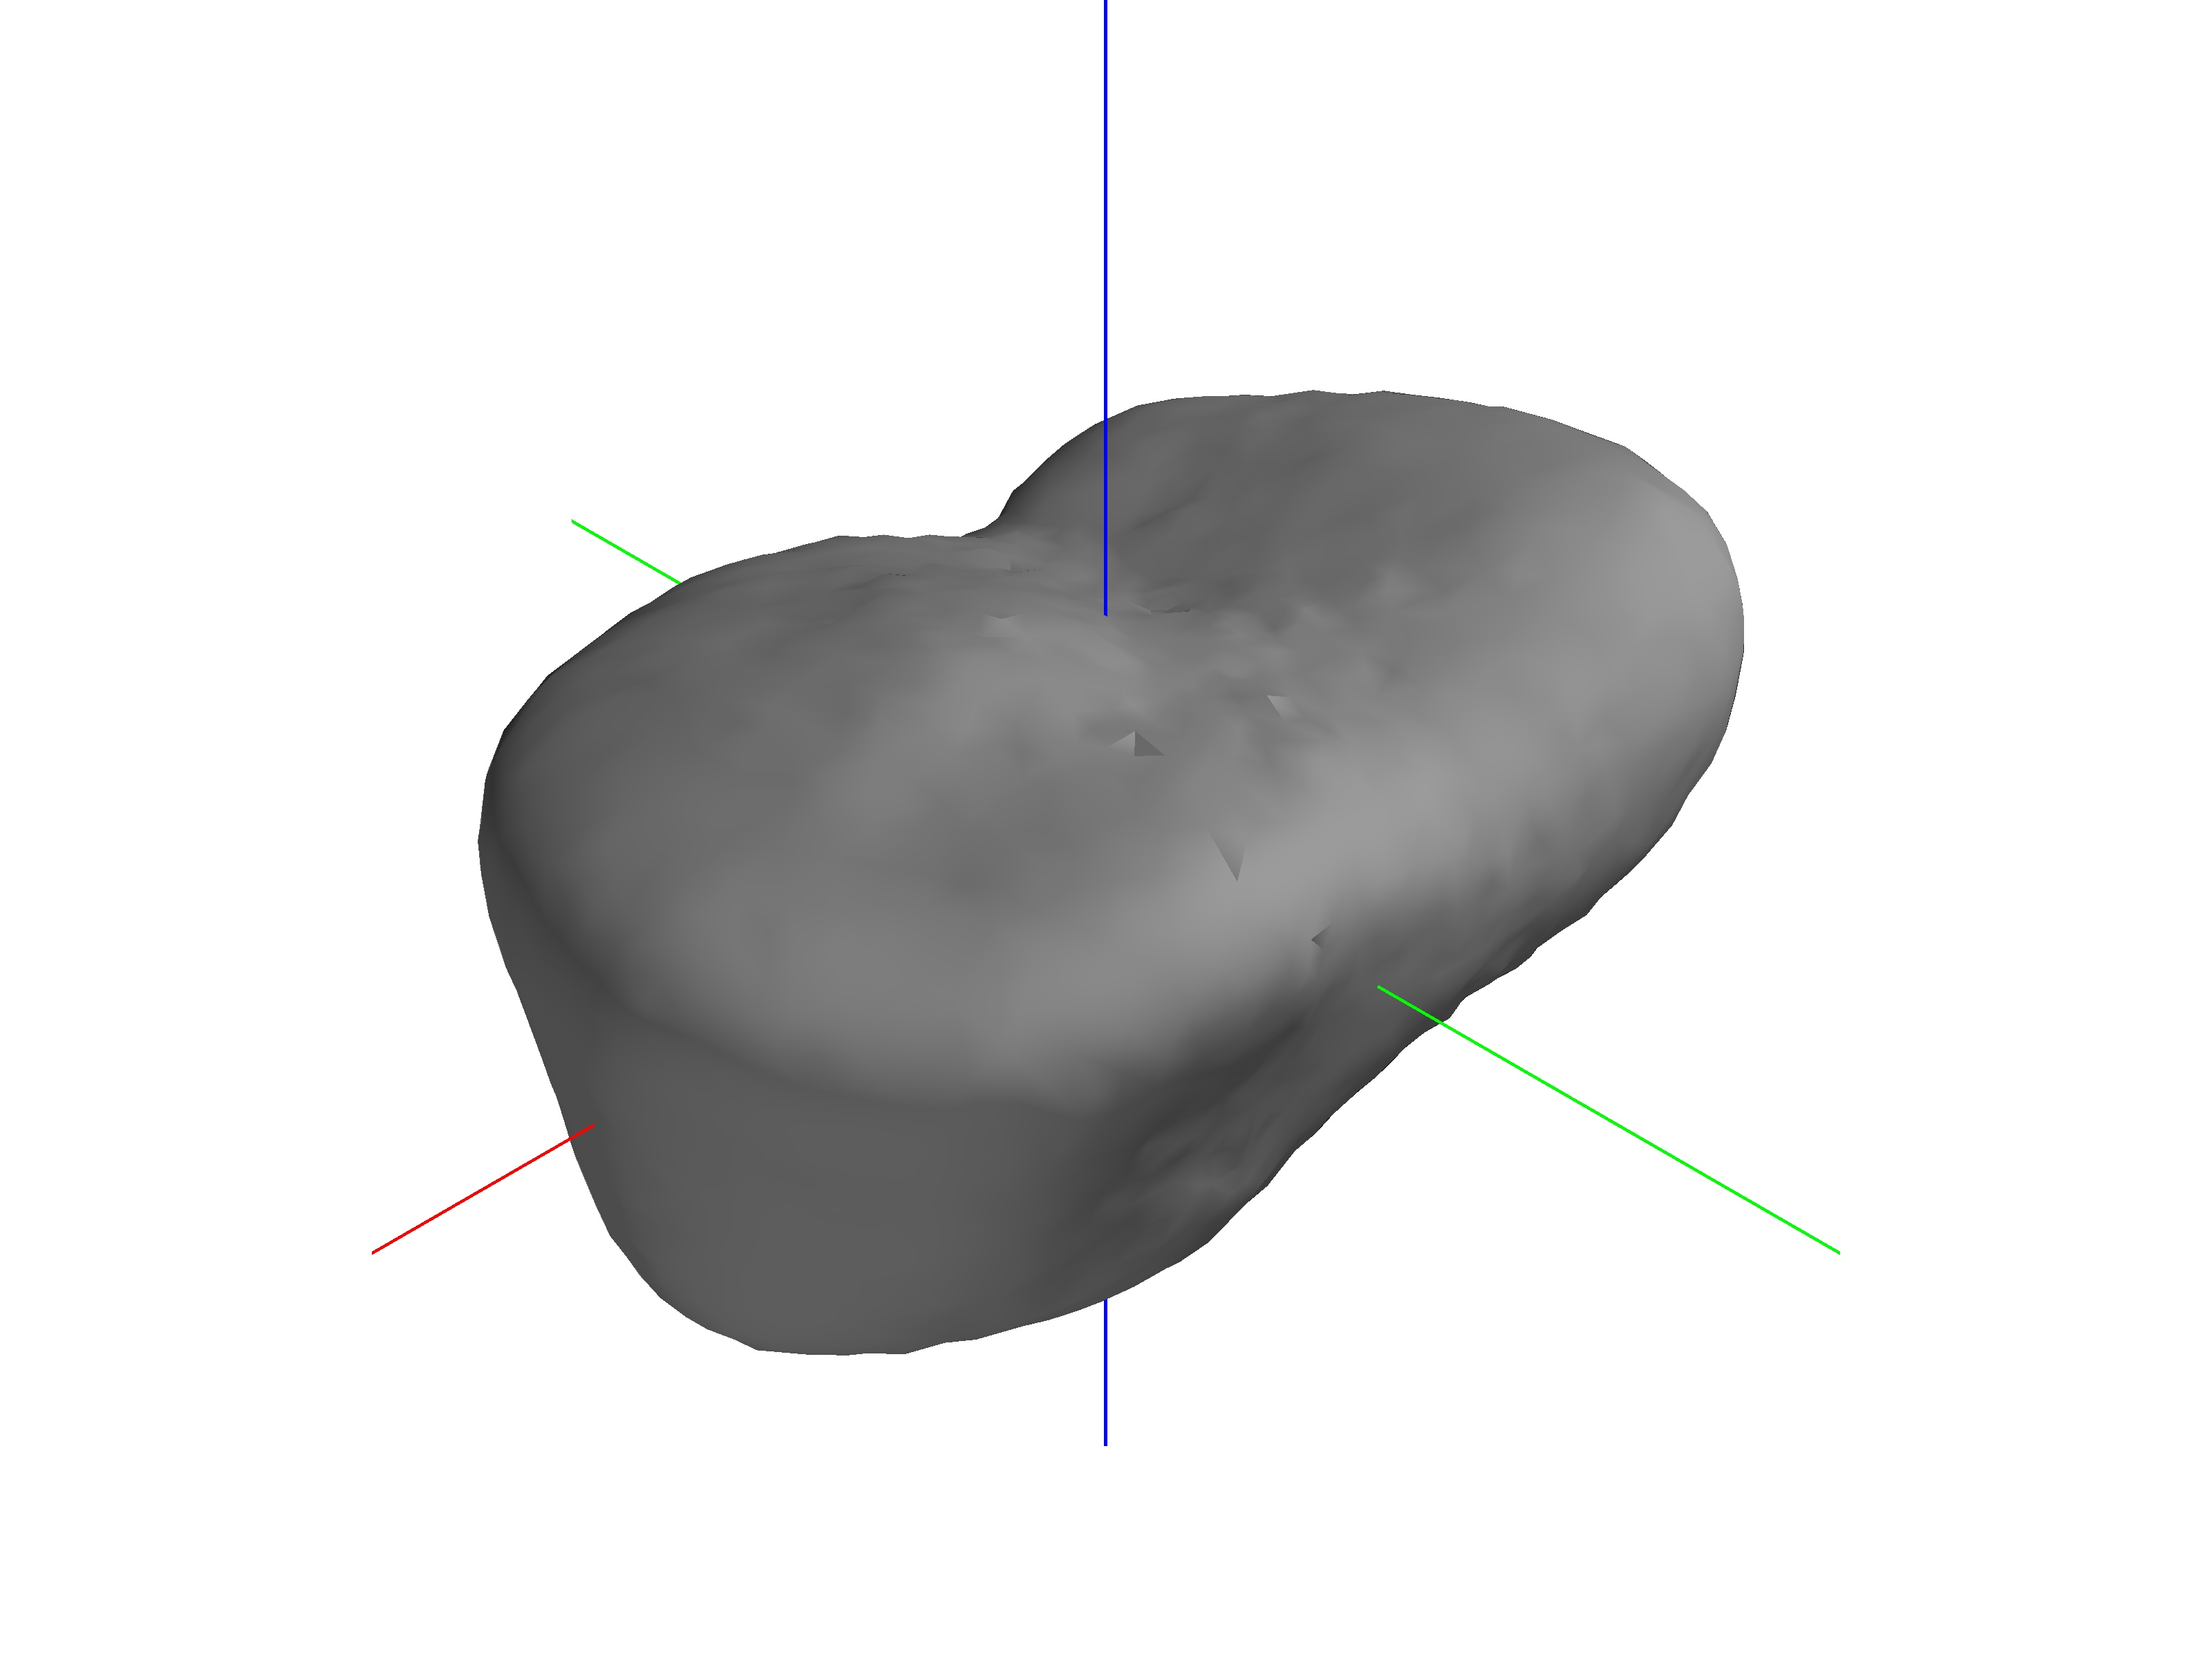
\includegraphics[width=0.5\textwidth,height=0.6\textheight,keepaspectratio]{figures/castalia/partial_2047.jpg}}{animation/castalia.u3d}

            \mediabutton[3Dgotoview=castalia:N]{\fbox{Next view}}
            \mediabutton[3Dgotoview=castalia:(Back)]{\fbox{Prev view}}
        \end{column}
        \begin{column}{0.5\textwidth}
            \centering
            \includemedia[
            label=castalia_reconstruction,
            3Dviews=animation/castalia.vws,
            width=0.5\textwidth,height=0.6\textheight,
            3Dmenu, 
            3Dc2c=-1 0 0,
            3Dcoo=0.04557958245277405 -0.03455224633216858 -0.017790749669075012,
            3Droo=4.029169586482155,
            3Dlights=Headlamp,
            % add3Djscript=animation/castalia.js
            ]{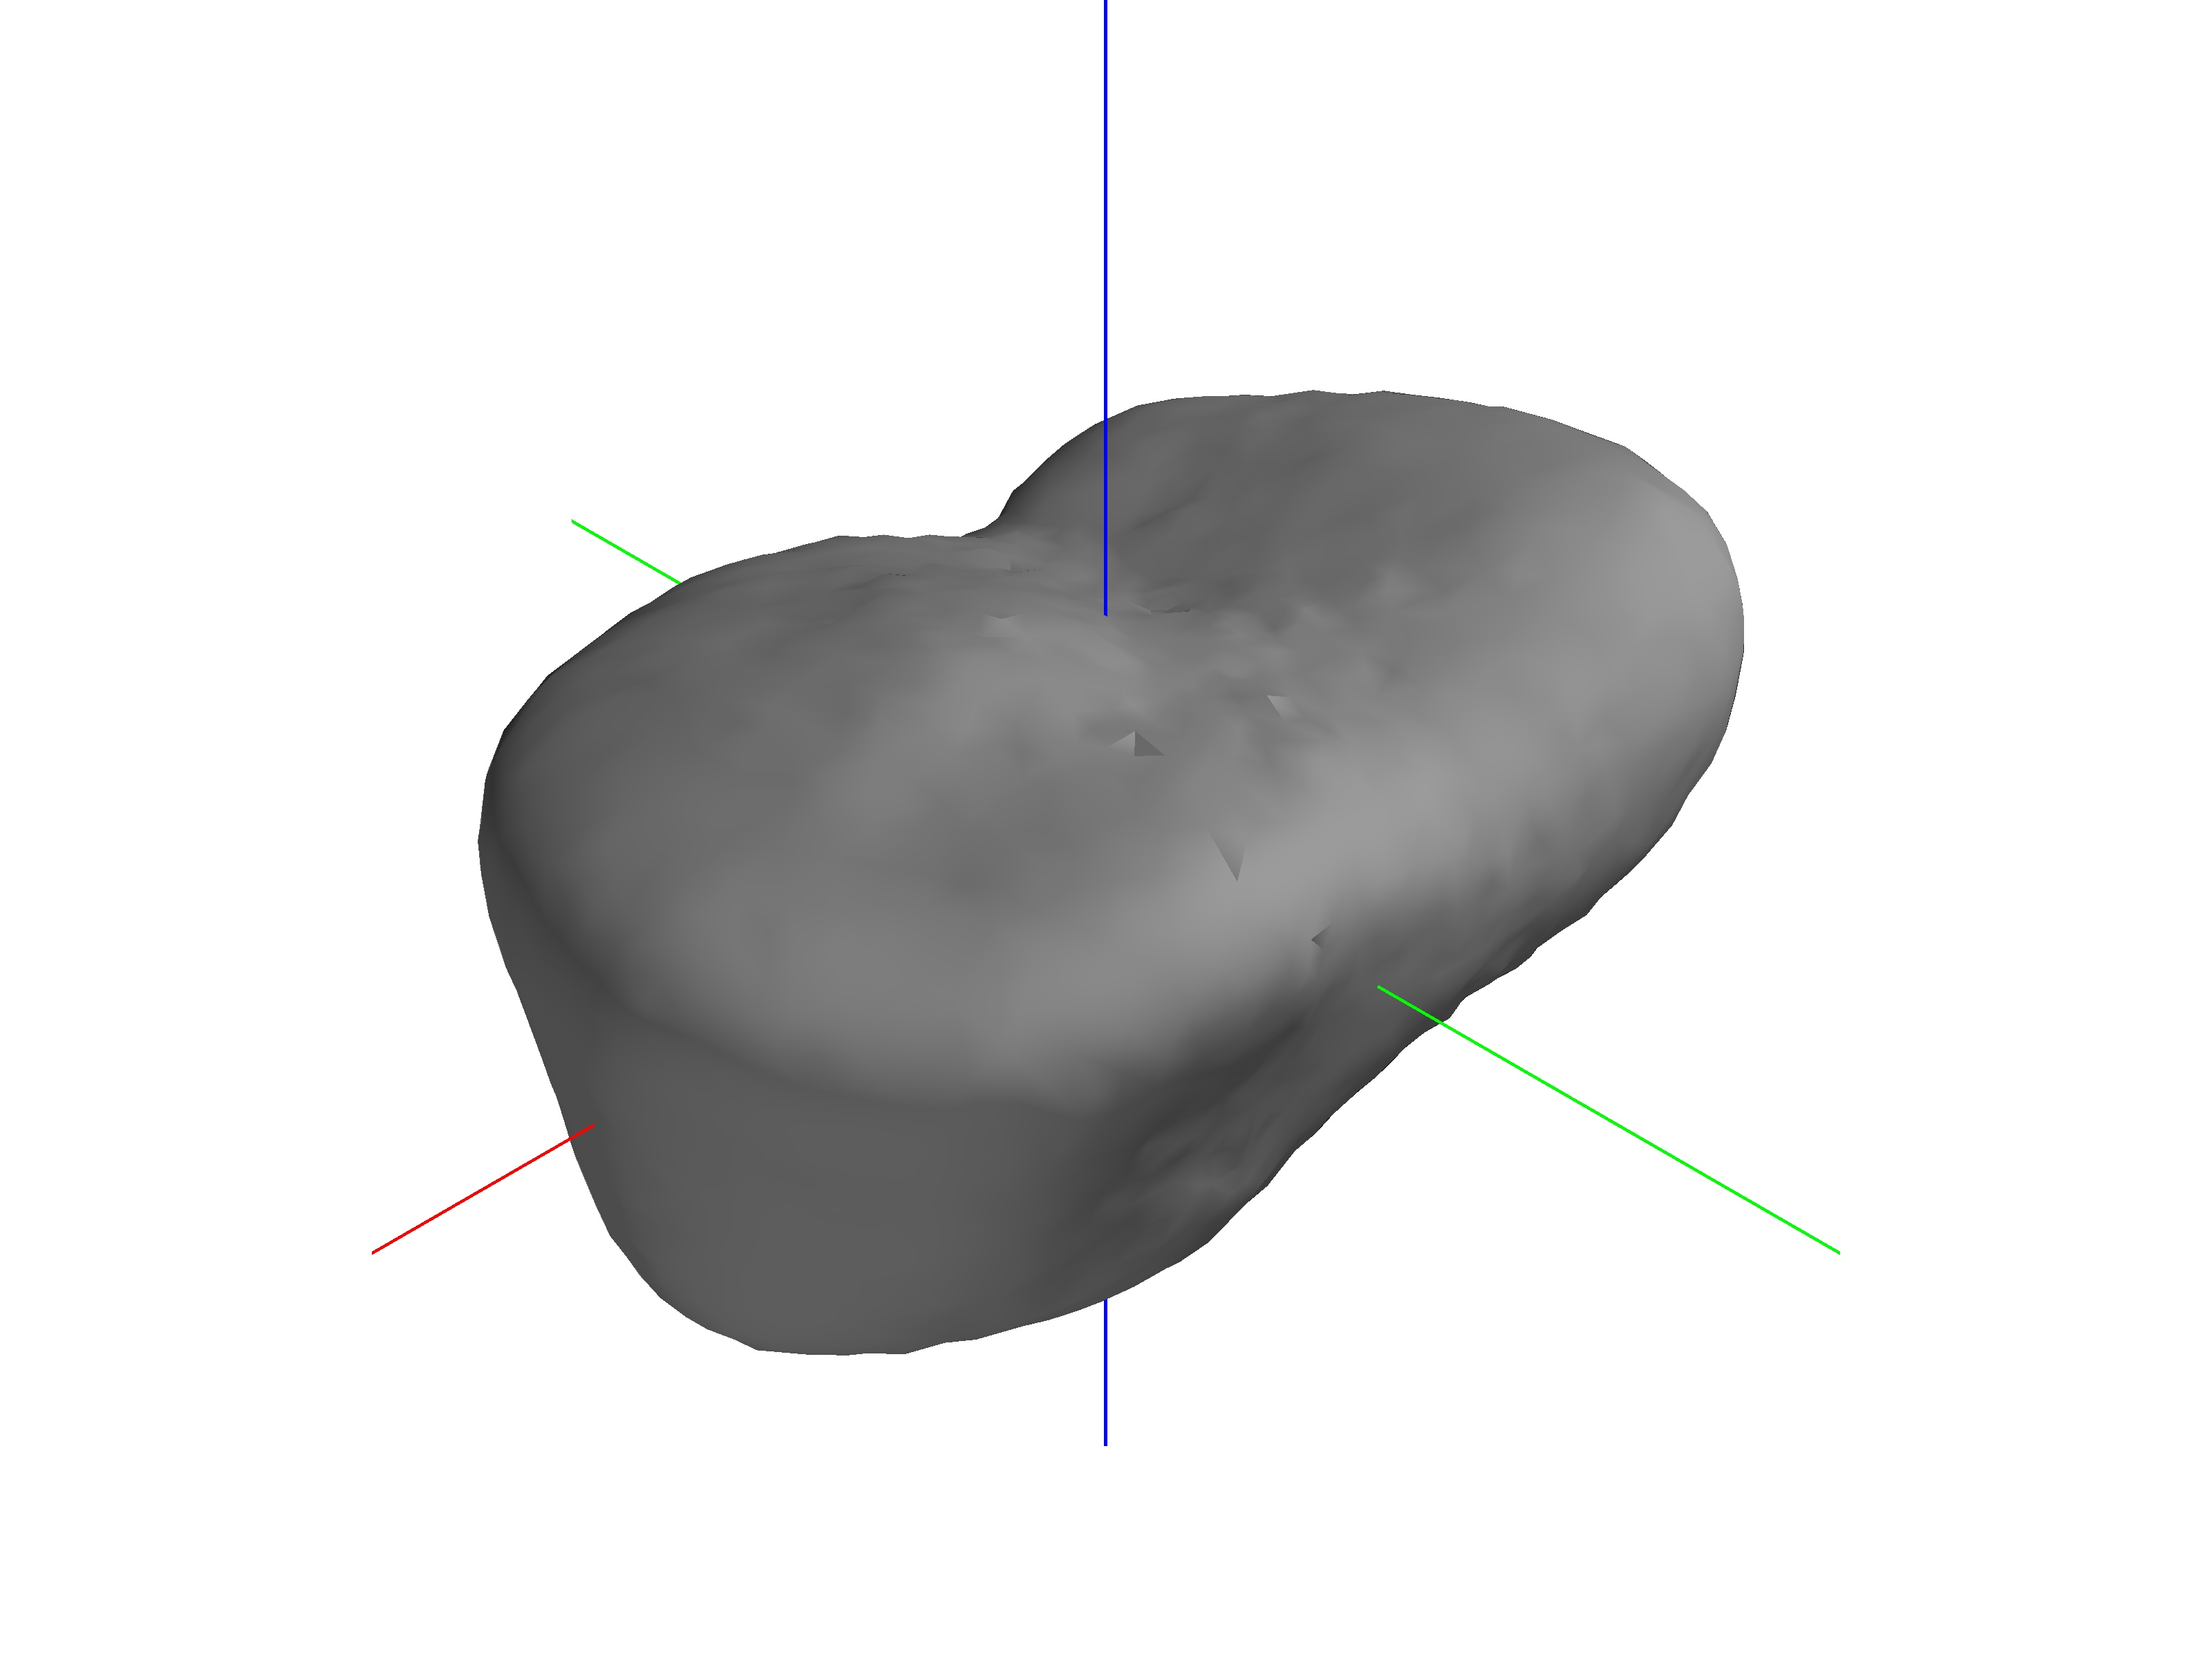
\includegraphics[width=0.5\textwidth,height=0.6\textheight,keepaspectratio]{figures/castalia/partial_2047.jpg}}{animation/castalia_reconstruction.u3d}

            \mediabutton[3Dgotoview=castalia_reconstruction:N]{\fbox{Next view}}
            \mediabutton[3Dgotoview=castalia_reconstruction:(Back)]{\fbox{Prev view}}
        \end{column}
    \end{columns}
\end{frame}

\begin{frame}{25143 Itokawa}
    \begin{center}
    \begin{columns}
        \begin{column}{0.5\textwidth}
            \centering
            \includemedia[
            label=itokawa,
            3Dviews=animation/itokawa.vws,
            width=0.5\textwidth,height=0.6\textheight,
            3Dmenu, 
            3Dc2c=-1 0 0,
            3Dcoo=-0.025140970945358276 0.002201750874519348 -0.002508975565433502,
            3Droo=1.32135384972625,
            3Dlights=Headlamp,
            % add3Djscript=animation/castalia.js
            ]{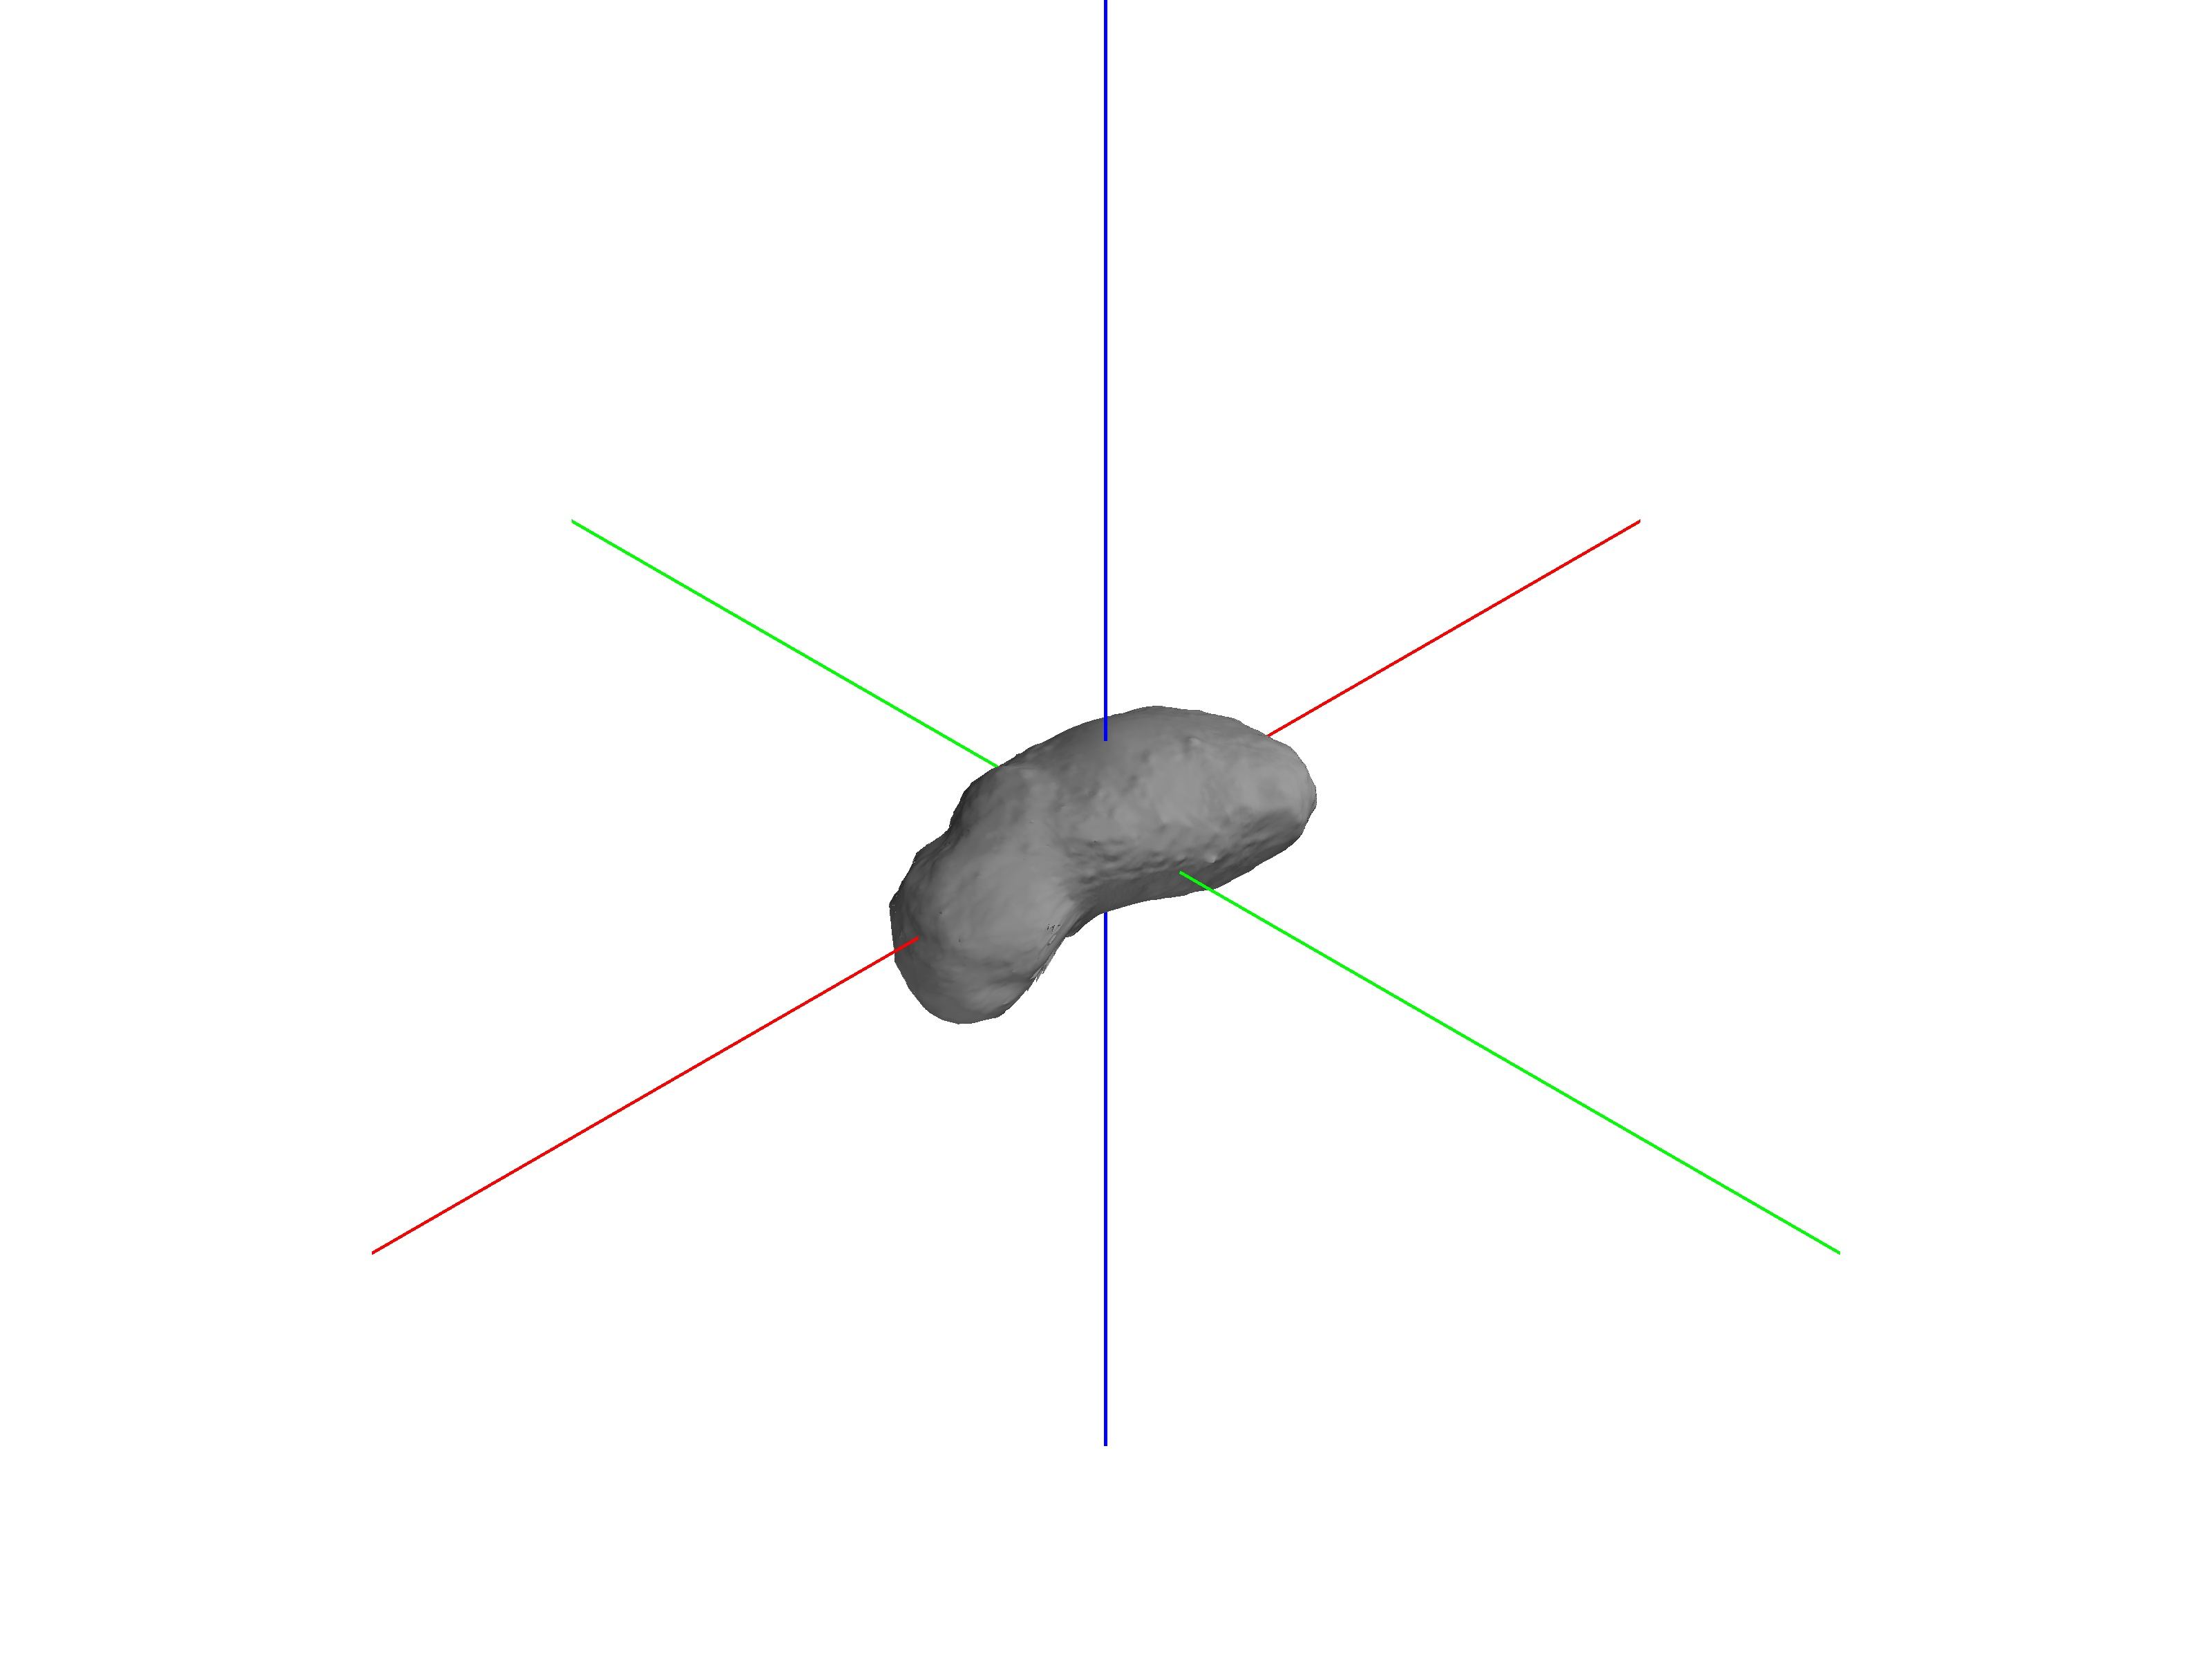
\includegraphics[width=0.5\textwidth,height=0.6\textheight,keepaspectratio]{figures/itokawa/partial_25349.jpg}}{animation/itokawa.u3d}

            \mediabutton[3Dgotoview=itokawa:N]{\fbox{Next view}}
            \mediabutton[3Dgotoview=itokawa:(Back)]{\fbox{Prev view}}
        \end{column}
        \begin{column}{0.5\textwidth}
            \centering
            \includemedia[
            label=itokawa_reconstruction,
            3Dviews=animation/itokawa.vws,
            width=0.5\textwidth,height=0.6\textheight,
            3Dmenu, 
            3Dc2c=-1 0 0,
            3Dcoo=-0.025140970945358276 0.002201750874519348 -0.002508975565433502,
            3Droo=1.32135384972625,
            3Dlights=Headlamp,
            % add3Djscript=animation/castalia.js
            ]{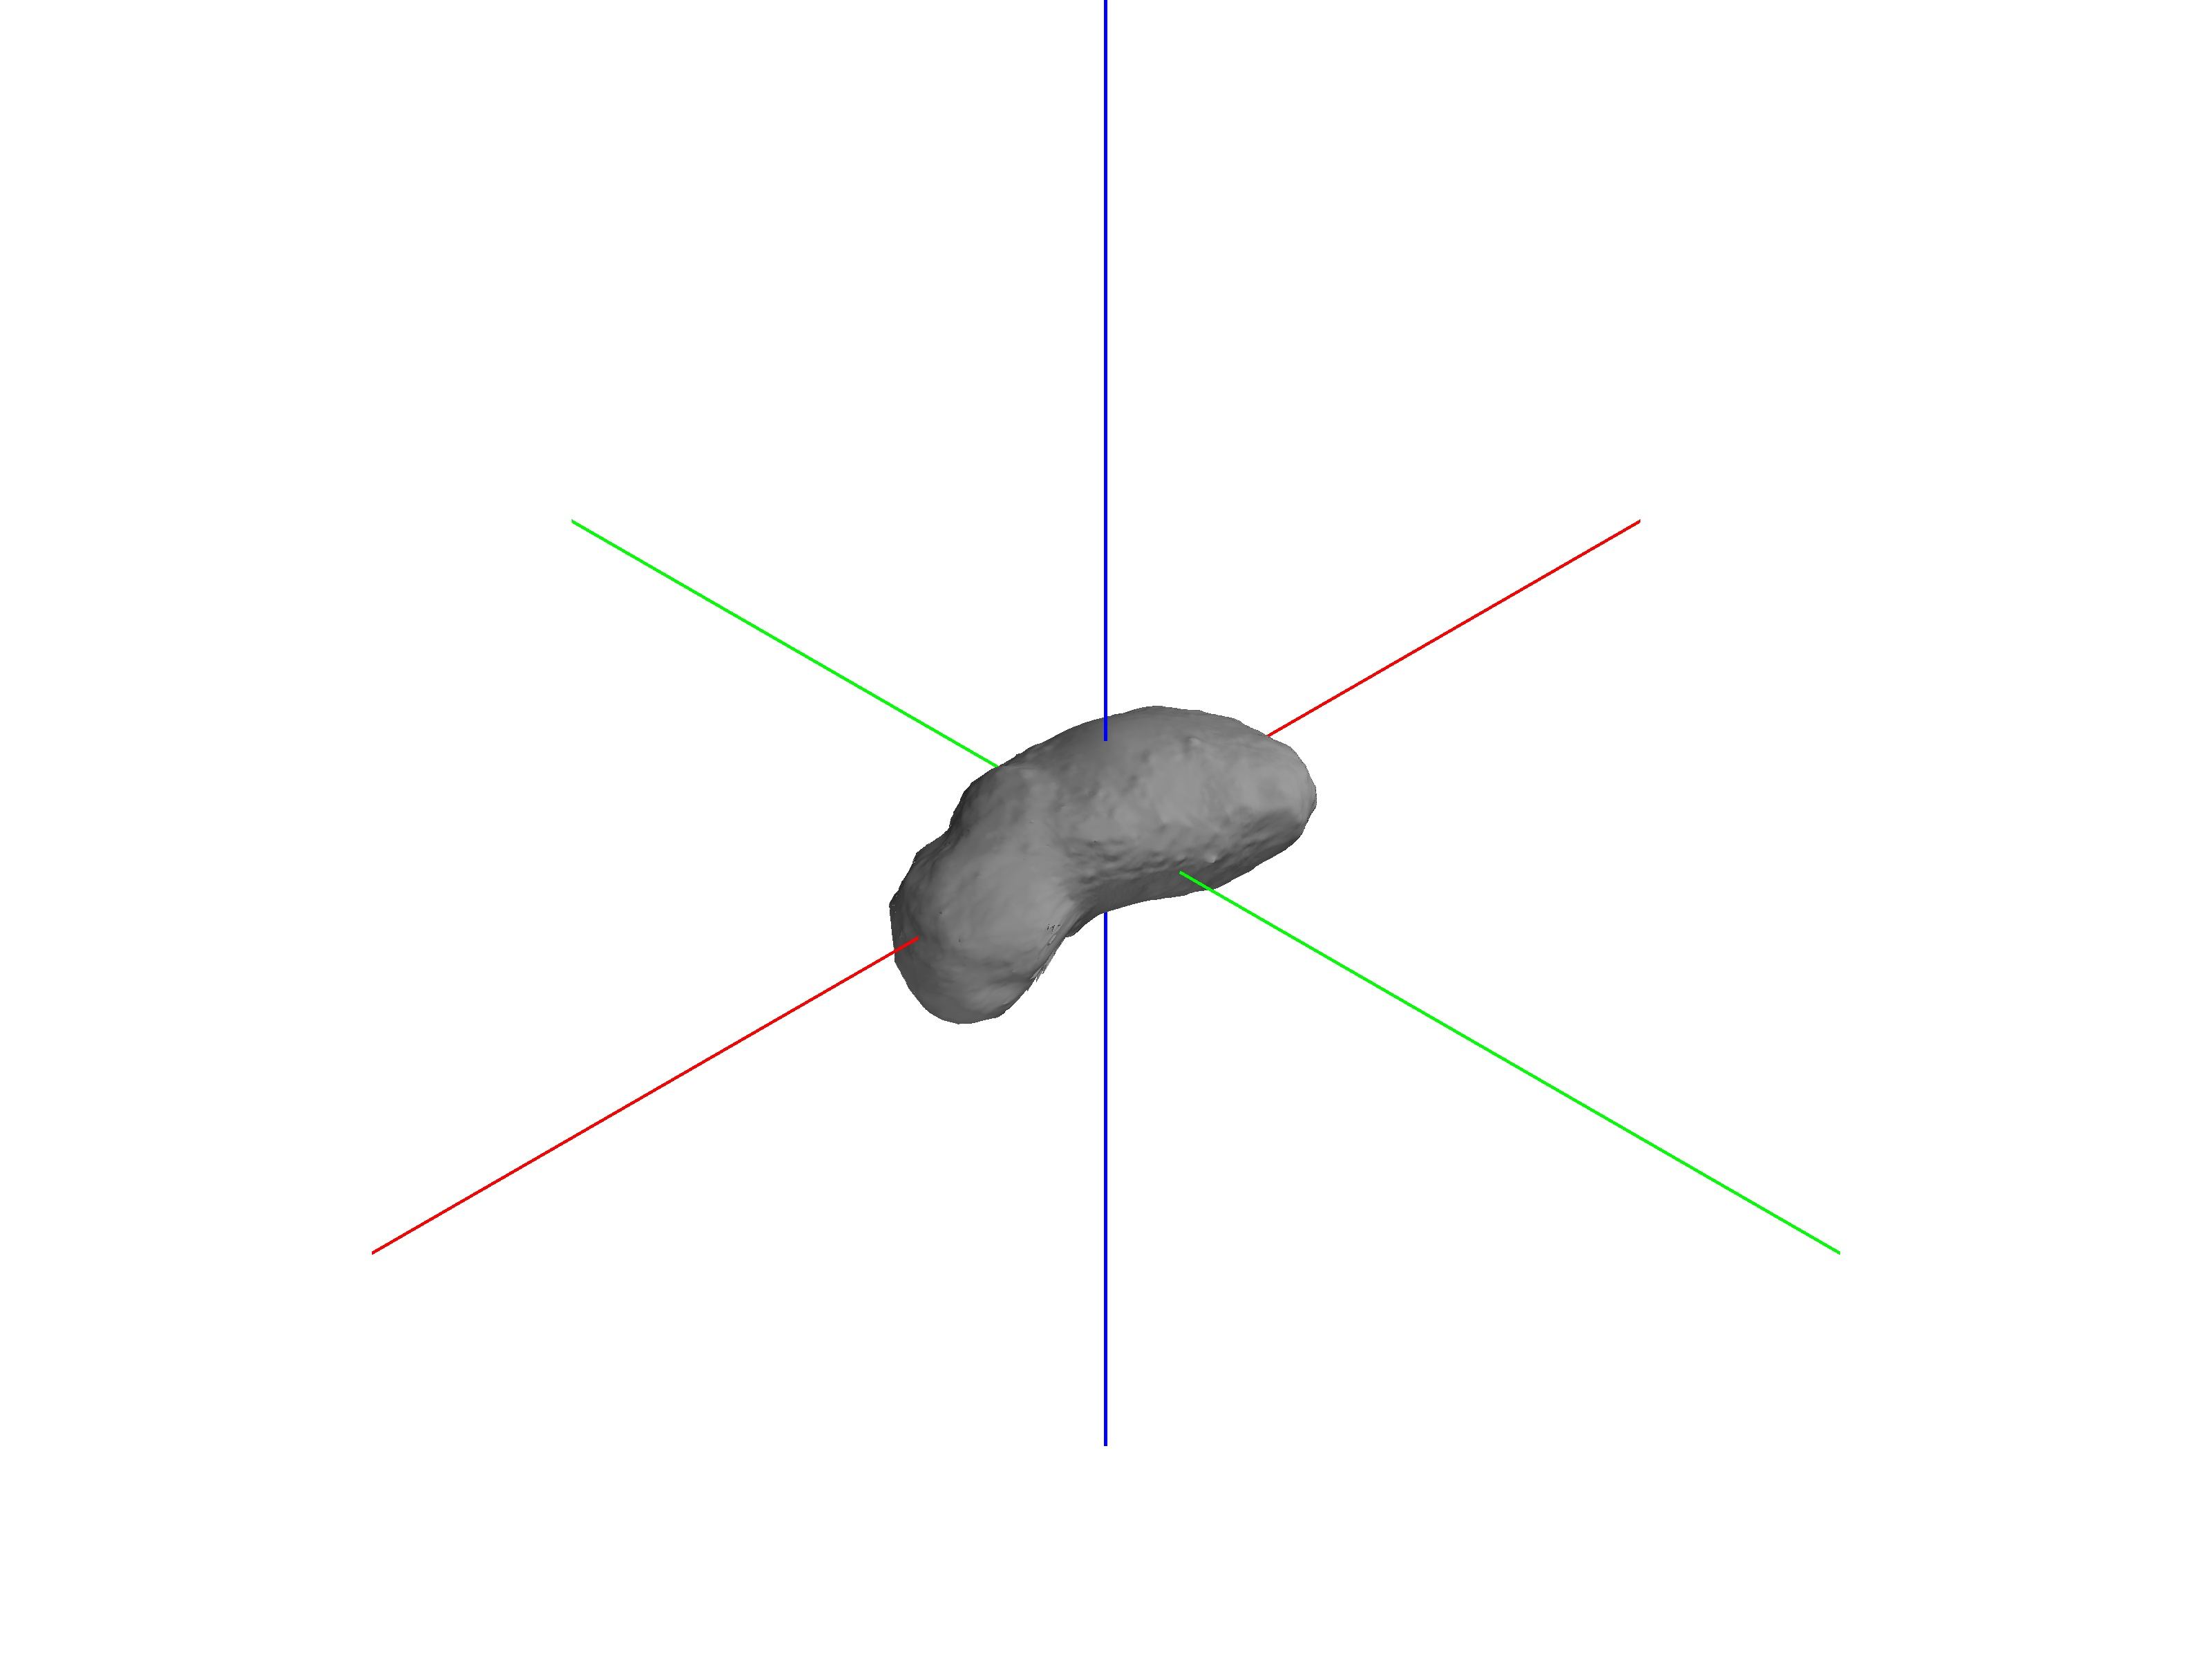
\includegraphics[width=0.5\textwidth,height=0.6\textheight,keepaspectratio]{figures/itokawa/partial_25349.jpg}}{animation/itokawa_reconstruction.u3d}

            \mediabutton[3Dgotoview=itokawa_reconstruction:N]{\fbox{Next view}}
            \mediabutton[3Dgotoview=itokawa_reconstruction:(Back)]{\fbox{Prev view}}
        \end{column}
    \end{columns}
\end{center}
\end{frame}
\section*{}
\subsection*{Conclusions}

\begin{frame}{Conclusions}
    \begin{itemize}
        \item Real time asteroid shape reconstruction 
        \item Each measurement is used to locally update the mesh
        \item Future Research Goals:
            \begin{itemize}
                \item Utilize state estimates directly in controller
                \item Design a trajectory to best reconstruct the shape
            \end{itemize}
    \end{itemize} 

    \begin{center}
        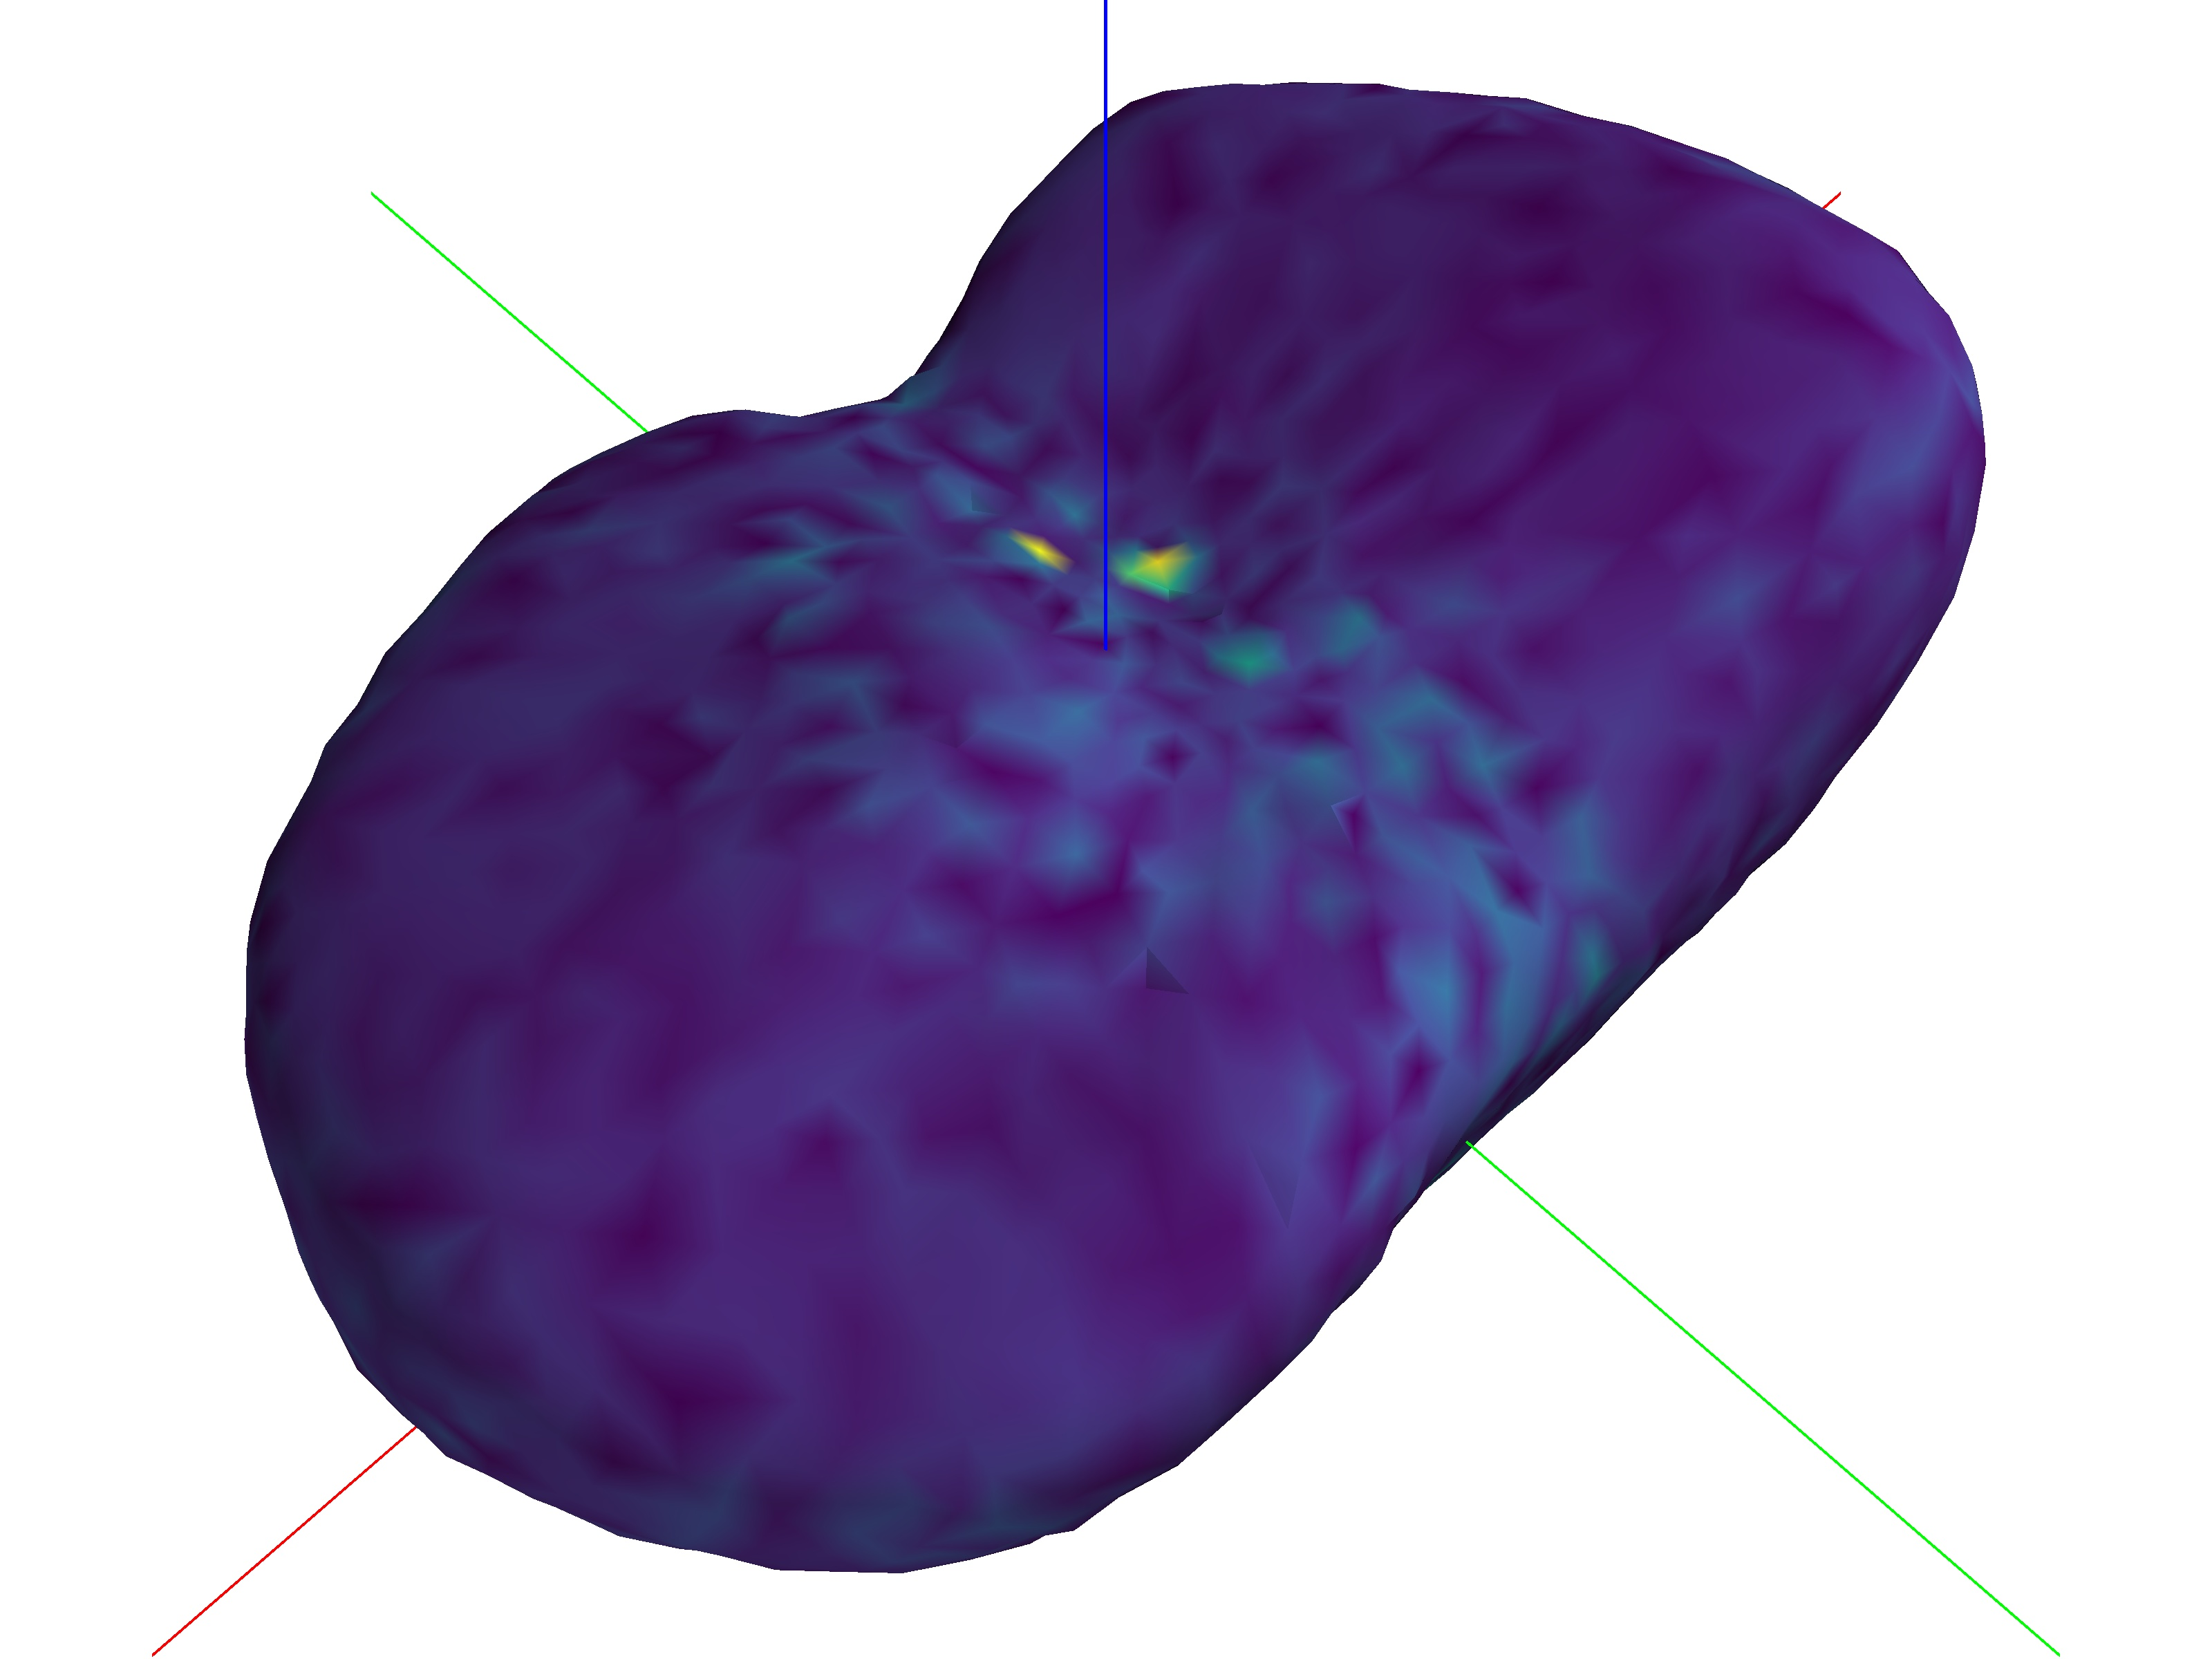
\includegraphics[width=0.5\textwidth,keepaspectratio]{figures/castalia/final_az=45_el=30.jpg}~
        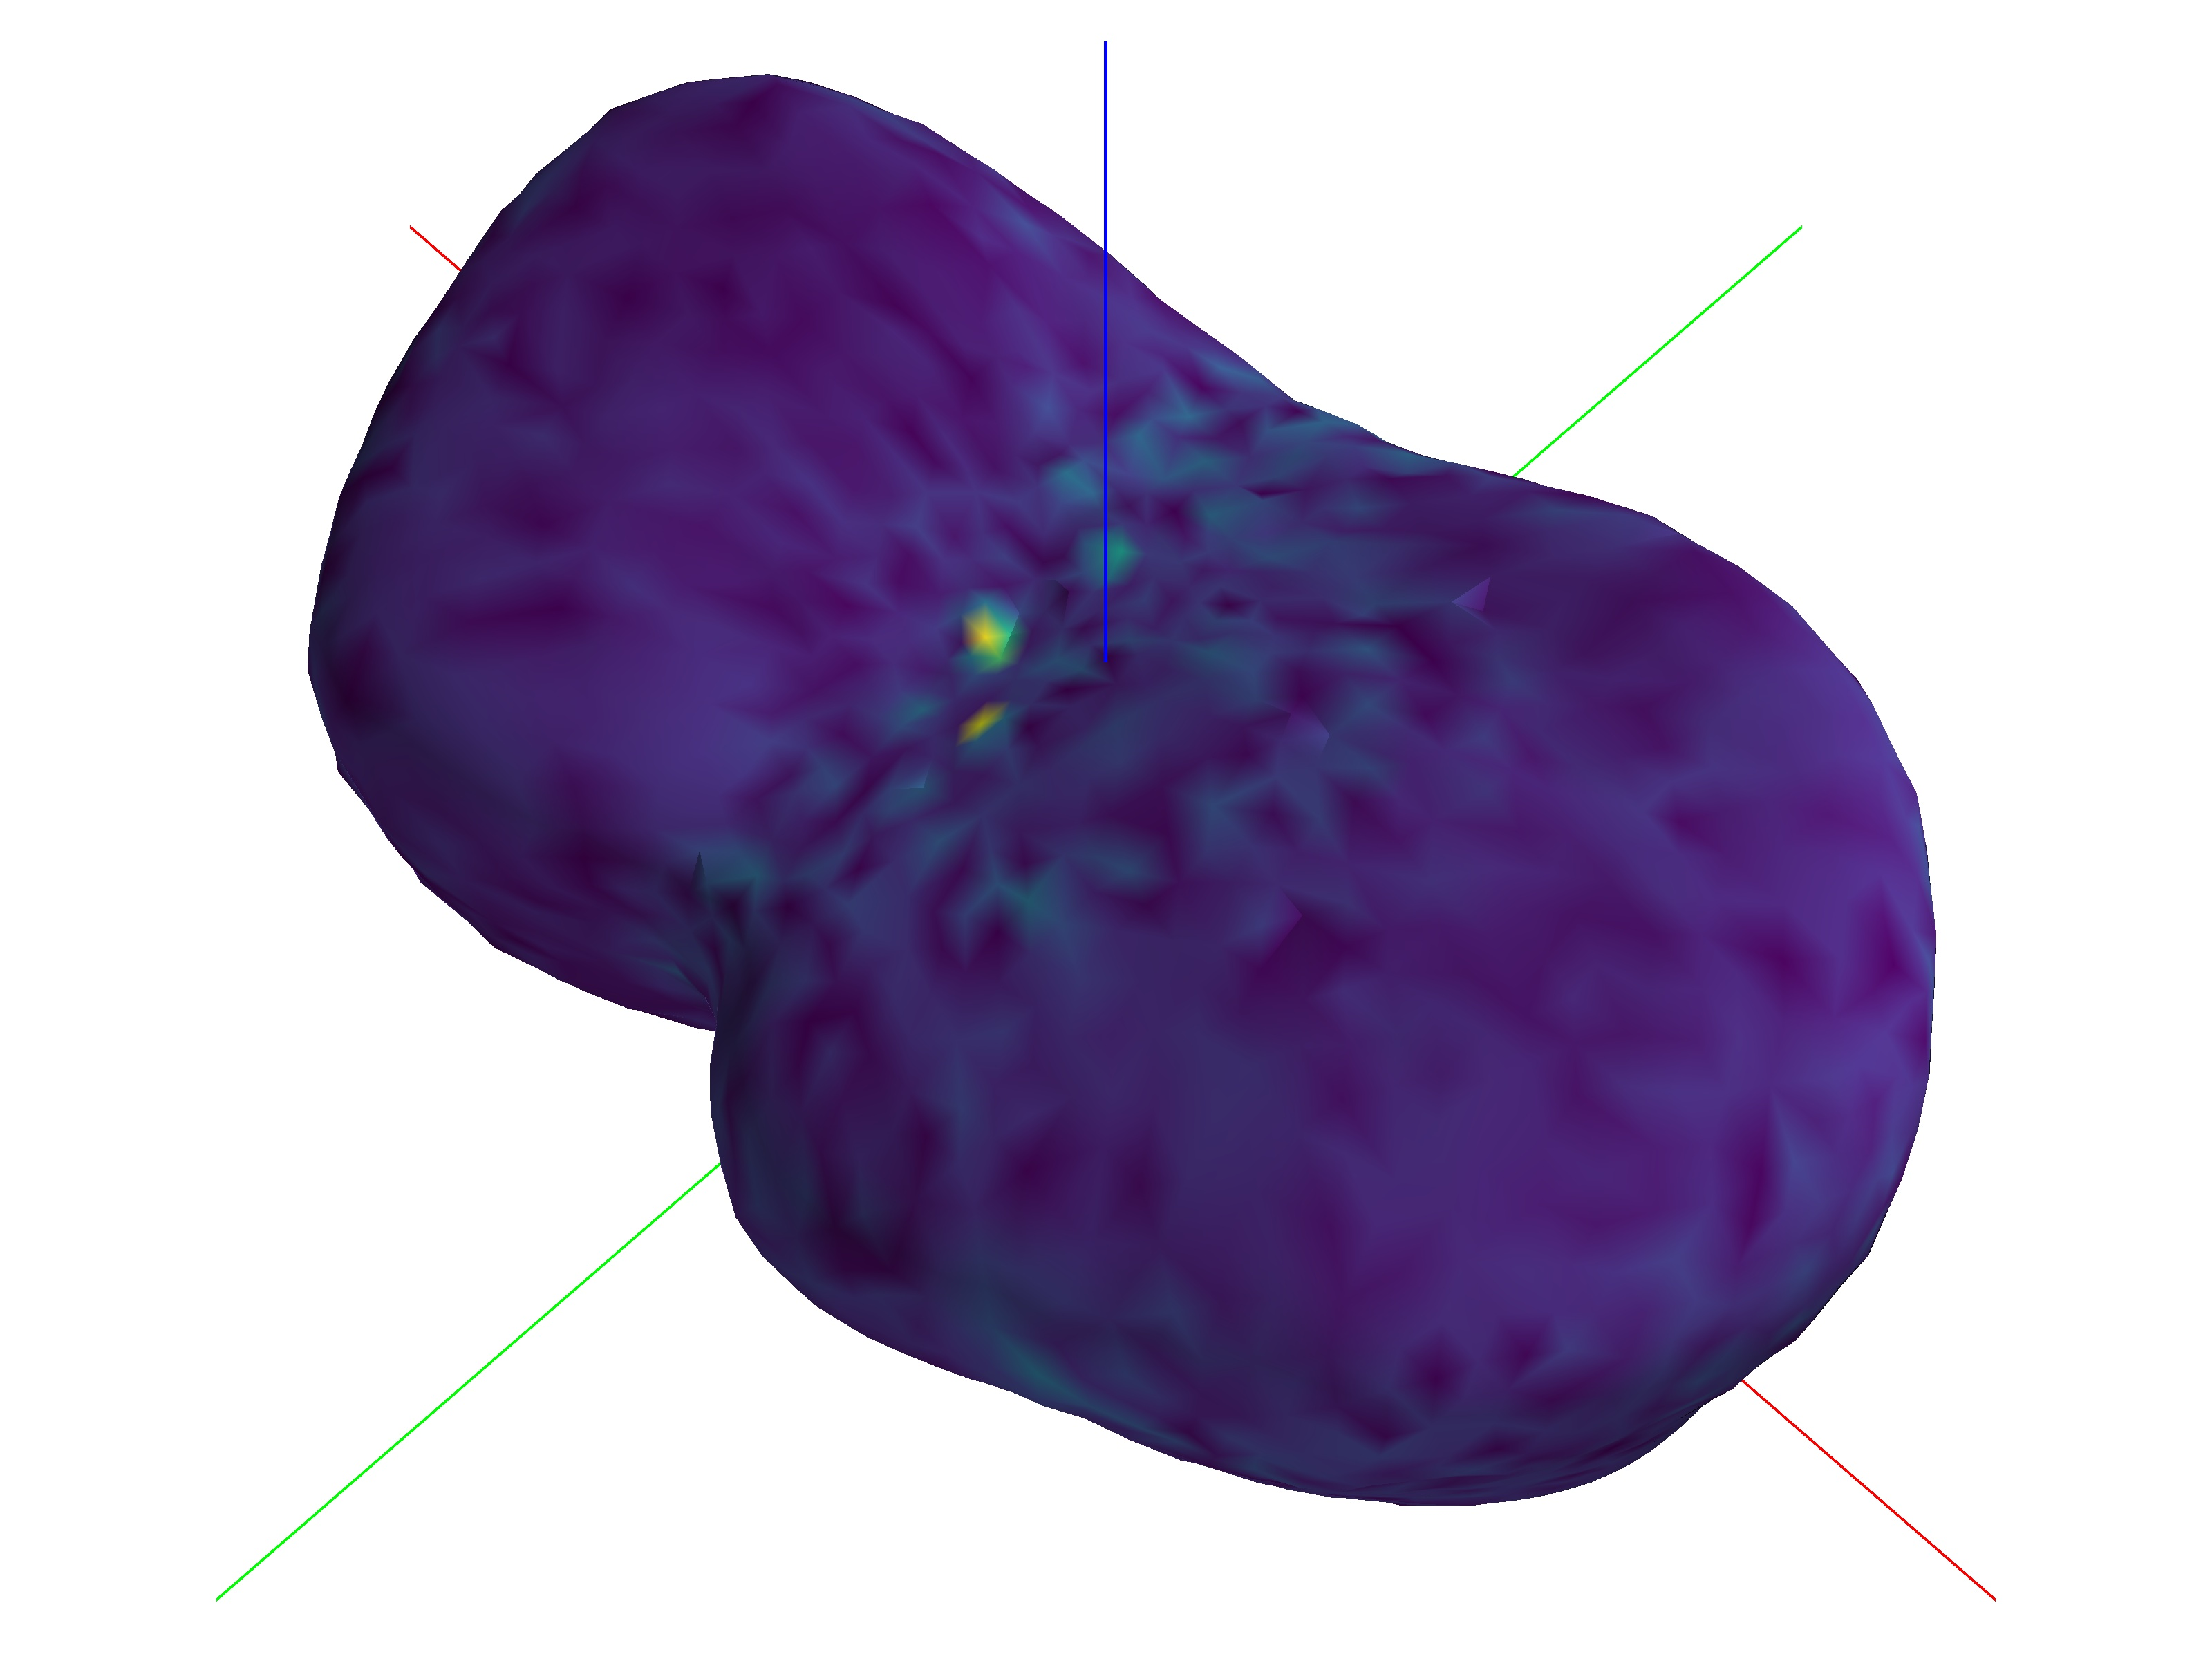
\includegraphics[width=0.5\textwidth, keepaspectratio]{figures/castalia/final_az=315_el=30.jpg}
    \end{center}
\end{frame}

\begin{frame}[c]{Thank you}
  \centering
  
  \textbf{\large Flight Dynamics \& Control Lab} \\
  Mechanical \& Aerospace Engineering \\
  School of Engineering \& Applied Science
  
  \begin{figure} %figure%
        
\includegraphics[width=0.75\textwidth]{gw_txh_2cs_pos}
    \end{figure}
  
  \url{https://fdcl.seas.gwu.edu}
\end{frame}
\end{document}

